% !TEX program = xelatex
\documentclass[UTF8]{ctexart}

\RequirePackage{inputenc}
\RequirePackage{fontspec}
\RequirePackage{xeCJK}

\RequirePackage{amsmath}
\RequirePackage{mhchem}
\RequirePackage{chemfig}
\RequirePackage{graphicx}

\RequirePackage{tikz}
\usetikzlibrary{calc} 

\RequirePackage{geometry}

\RequirePackage{siunitx}

\RequirePackage[hidelinks]{hyperref}

\setmainfont{Times New Roman}

\setCJKmainfont{等线}
\setCJKsansfont{等线}
\setCJKmonofont{等线}

\newcommand{\rnum}[1]{\uppercase\expandafter{\romannumeral #1\relax}}

\newcommand{\LiValence}[3]
{
    \overset{\texttt{\tiny #1}\text{\tiny #2}}{\ce{#3}}
}

\newcommand{\LiDrawContainer}[6][solid]
{
    \coordinate (A1) at #2;
    \coordinate (A2) at #3;
    \coordinate (B1) at ($#2+(0,#4)$);
    \coordinate (B2) at ($#3+(0,#4)$);

    \draw (A1)--(B1);
    \draw[#1] (B2)--(A2);
    \draw (B1)--(B2);

    \node at($0.5*(B1)+0.5*(B2)+(0,#5)$) {#6};
}

\geometry
{
    left=1.25in,
    right=1.25in,
    top=1in,
    bottom=1in
}

\title{化学笔记}
\author{李宇轩}
\date{2019.08.26}

\begin{document}
\maketitle

\newpage

\tableofcontents

\newpage

\setlength{\parindent}{0pt}

\section{化学计量}

\subsection{物质的量}
    物质的量衡量了一定量粒子的集合体中所含粒子的数量,通常用符号$n$表示,单位是\si{mol}。\\[3mm]
    物质的量的单位称为摩尔,其定义为$0.012$\si{kg}~的\ce{^12C}中含有的碳原子数目。\\[3mm]
    这一数目称为阿伏伽德罗常数,记作$N_A$:
    \begin{large}
        \begin{equation*}
            N_A=6.02\times 10^{23}~~\si{1/mol}
        \end{equation*}
    \end{large}\\
    物质的量的定义如下:
    \begin{large}
        \begin{equation*}
            n=\frac{N}{N_A}
        \end{equation*}
    \end{large}\\
    物质的量($n$)定义为物质所含微粒数($N$)与阿伏伽德罗常数($N_A$)的比。\\[3mm]
    物质的量是七个基本物理量之一,物质的量是一个将微观和宏观联系起来的物理量。

\subsubsection{摩尔质量}
    摩尔质量衡量了单位物质的量的物质的质量,通常用符号$M$表示,单位是\si{g/mol}。\\[3mm]
    摩尔质量的定义如下:
    \begin{large}
        \begin{equation*}
            M=\frac{m}{n}
        \end{equation*}
    \end{large}\\
    摩尔质量定义为物质的质量与物质的量的比值。\\[3mm]
    摩尔质量是有单位的,式量是没有单位的,前者在数值上等于后者。\\[3mm]
    例如~\ce{O2}的式量为$32$,而~\ce{O2}的摩尔质量为$32$\si{g/mol}。\\[3mm]
    例如~\ce{CuSO4}的式量为$160$,而~\ce{CuSO4}的摩尔质量为$160$\si{g/mol}。

\subsubsection{摩尔体积}
    摩尔体积衡量了单位物质的量的物质的体积,通常用符号$V_m$表示,单位是\si{L/mol}。\\[3mm]
    摩尔体积的定义如下:
    \begin{large}
        \begin{equation*}
            V_m=\frac{V}{n}
        \end{equation*}
    \end{large}\\
    摩尔体积定义为物质的体积与物质的量的比值。\\[3mm]
    摩尔体积用于气体和液体时常用\si{L/mol},摩尔体积用于固体时常用\si{cm^3/mol}。

\newpage

\subsubsection{摩尔浓度}
    摩尔浓度衡量了单位体积的溶液所含溶质的物质的量,通常用符号$c$表示,单位是\ce{mol/L}。\\[3mm]
    摩尔浓度的定义如下:
    \begin{large}
        \begin{equation*}
            c=\frac{n}{V}
        \end{equation*}
    \end{large}\\
    摩尔浓度定义为为溶质的物质的量和溶液体积的比值。\\[3mm]
    摩尔浓度有助于定量实验的进行,因为化学的定量实验中我们更为关心的是反应物的物质的量,
    若已知所需溶液的摩尔浓度,则可以通过测量溶液的体积,从而计算得知溶质的物质的量。\\[8mm]
    质量浓度衡量了单位体积的溶液所含溶质的质量,单位是\si{g/L}。\\[3mm]
    质量分数衡量了单位质量的溶液所含溶质的质量,是一个无量纲量。\\[3mm]
    若我们分布使用符号:$M$表示溶质的摩尔质量,$\omega$表示溶质的质量分数,$\rho$表示溶液密度。\\[3mm]
    摩尔浓度和质量分数的关系如下:
    \begin{large}
        \begin{equation*}
            c=\frac{\rho\cdot\omega}{M}
        \end{equation*}
    \end{large}\\
    因为溶液中的溶质的物质的量既可以表达为:
    \setcounter{equation}{0}
    \begin{align}
        n=c\cdot V
    \end{align}\\
    同时溶液中的溶质的物质的量也可以表达为:
    \begin{align}
        n=\frac{\rho\cdot\omega}{M}\cdot V
    \end{align}\\
    在上式中,$\rho\cdot V$代表溶液的质量,$\rho\cdot V\cdot\omega$代表溶质的质量,故该等式成立。\\[3mm]
    两式联立,消去溶液的体积$V$,即可证明摩尔浓度和质量分数的关系。\\[3mm]

\newpage

\subsubsection{阿伏伽德罗定律}
    \textbf{阿伏伽德罗定律:}在相同的温度和压强下,相同体积的任何气体都含有相同数目的分子。\\[5mm]
    决定物质体积的因素有三个:\\[3mm]
    1.物质所含微粒的多少。\\[3mm]
    2.物质所含微粒的大小。\\[3mm]
    3.物质所含微粒的间距。\\[6mm]
    对于一定量的固体来说,其微粒的间距很小,因此其体积主要由微粒的大小决定。\\[3mm]
    对于一定量的液体来说,其微粒的间距很小,因此其体积主要由微粒的大小决定。\\[3mm]
    对于一定量的气体来说,其微粒的间距很大,因此其体积主要由微粒的间距决定。\\[6mm]
    一般来说,温度越高,气体的分子间距越大,温度越低,气体的分子间距越小。\\[3mm]
    一般来说,压强越大,气体的分子间距越小,压强越小,气体的分子间距越大。\\[3mm]
    因此当温度和压强一定时,对于相同量的任何气体,其体积均为一相同的定数值。\\[6mm]
    任何气体在$0$\si{\degreeCelsius}和$1.01\times 10^5$\si{Pa}的标准状况下:
    \begin{large}
        \begin{equation*}
            V_m=22.4\si{L/mol}
        \end{equation*}
    \end{large}\\
    任何气体在标准状况下的摩尔体积为定值,这一定值称为气体摩尔体积。

\newpage

\subsection{热化学反应方程式}
    热化学反应方程式可以用于表示反应热和化学反应间关系的一种化学方程式。\\[3mm]
    热化学反应方程式的例子:
    \begin{center}
        \ce{2H2(g) + O2(g) -> 2H2O(l)\; + 571.6\si{kJ}}\\[3mm]
        \ce{2H2(g) + O2(g) -> 2H2O(g) + 483.6\si{kJ}}\\[6mm]
    \end{center}
    热化学反应方程式需要注意以下三点:\\[3mm]
    1.热化学反应方程式中的系数直接代表对应物质的物质的量,因而可以出现分数。\\[3mm]
    2.热化学反应方程式需要标注反应产生或吸收的热量。\\[3mm]
    3.热化学反应方程式需要标注反应物和生成物的物态。\\[3mm]
    4.热化学反应方程式可以不标注反应条件。\\[6mm]
    在反应中如果反应产生热量,则标记热量为正。\\[3mm]
    在反应中如果反应产生热量,则标记热量为负。\\[3mm]
    标注反应物和生成物的物态时可以使用以下简写:\vspace{5pt}
    \begin{table}[h]
        \begin{center}
            \begin{tabular}{p{80pt}|p{80pt}|p{80pt}}
                \hline
                物态&简写&含义\\ \hline
                气体&\ce{H2O}(g)&gas\\ \hline
                液体&\ce{H2O}(l)&liquid\\ \hline
                固体&\ce{H2O}(s)&solid\\ \hline
                溶液&\ce{NaCl}(aq)&aqua\\ \hline
            \end{tabular}
        \end{center}
        \caption{热化学反应方程式中的物态简写}
    \end{table}\\
    之所以需要标注物态,是因为不同物态间存在能量上的差异,会影响产生或吸收的热量大小。\\[3mm]
    在上方的例子中,由于液态的水需要吸收能量才能变为气态的水:\\[3mm]
    因此液态的水能量较低,故燃烧生成液态的水时需要放出更多的热量。\\[3mm]
    因此气态的水能量较高,故燃烧生成气态的水时只能放出更少的热量。

\newpage

\subsubsection{中和热}
    中和热指的是稀溶液的酸碱中和所放出的热量。\\[3mm]
    中和热需要控制反应得到的水为$1$\si{mol}。\\[3mm]
    \textbf{1.一元强弱和一元强碱}\\[3mm]
    盐酸和氢氧化钠的中和反应:
    \begin{center}
        \ce{HCl(aq) + NaOH(aq) -> NaCl(aq) + H2O(l) + 57.3\si{kJ}}\\[3mm]
    \end{center}
    盐酸和氢氧化钾的中和反应:
    \begin{center}
        \ce{HCl(aq) + NaOH(aq) -> NaCl(aq) + H2O(l) + 57.3\si{kJ}}\\[3mm]
    \end{center}
    强酸和强碱中和反应的实质:
    \begin{center}
        \ce{H+(aq) + OH-(aq) -> H2O(l) + 57.3\si{kJ}}\\[3mm]
    \end{center}
    由此可见,一元强酸和一元强碱的中和热恒为$\Delta Q=57.3$\si{kJ}。\\[8mm]
    \textbf{2.一元弱酸和一元强碱}\\[3mm]
    醋酸和氢氧化钠的中和反应:
    \begin{center}
        \ce{HAc(aq) + NaOH(aq) -> NaAc(aq) + H2O(l) + 56.0\si{kJ}}\\[3mm]
    \end{center}
    氢氟酸和氢氧化钠的中和反应:
    \begin{center}
        \ce{HF(aq) + NaOH(aq) -> NaF(aq) + H2O(l) + 67.7\si{kJ}}\\[3mm]
    \end{center}
    大部分弱酸的电离需要吸收热量,故大部分一元弱酸和一元强碱的中和热$\Delta Q<57.3$\si{kJ}。\\[3mm]
    少部分弱酸的电离放出吸收热量,故少部分一元弱酸和一元强碱的中和热$\Delta Q>57.3$\si{kJ}。\\[8mm]
    \textbf{3.多元弱酸和一元强碱}\\[3mm]
    二元弱酸和一元强碱的中和热:
    \begin{large}
        \begin{equation*}
            \Delta Q=\frac{2\times 57.3~\si{kJ}-(\Delta Q_1+\Delta Q_2)}{2}
        \end{equation*}
    \end{large}\\
    三元弱酸和一元强碱的中和热:
    \begin{large}
        \begin{equation*}
            \Delta Q=\frac{3\times 57.3~\si{kJ}-(\Delta Q_1+\Delta Q_2+\Delta Q_3)}{3}
        \end{equation*}
    \end{large}\\
    其中符号$\Delta Q_1,\Delta Q_2,\Delta Q_3$分别代表电离出第一个\ce{H+}、第二个\ce{H+}、第三个\ce{H+}时吸收的热量。

\newpage

\subsubsection{燃烧热}
    燃烧热指的是在$25$\si{\degreeCelsius}和$101$\si{kPa}时,可燃物完全燃烧生成稳定的化合物时放出的热量。\\[3mm]
    燃烧热需要控制可燃物为$1$\si{mol}。\\[3mm]
    一氧化碳在氧气中的燃烧:
    \begin{center}
        \ce{CO(g) + \dfrac{1}{2}O2(g) -> CO2(g) + 283.3\si{kJ}}\\[4mm]
    \end{center}
    氢气在氧气中的燃烧:
    \begin{center}
        \ce{H2(g) + \dfrac{1}{2}O2(g) -> H2O(l) + 285.5\si{kJ}}\\[4mm]
    \end{center}
    甲烷在氧气中的燃烧:
    \begin{center}
        \ce{CH4(g) + 2O2(g) -> CO2(g) + 2H2O(l) + 890.3\si{kJ}}\\[4mm]
    \end{center}
    燃烧热定义中的稳定包含两个方面:\\[3mm]
    1.化学状态稳定:例如甲烷的燃烧中,生成二氧化碳属于稳定,生成一氧化碳属于不稳定。\\[3mm]
    2.物理状态稳定:例如甲烷的燃烧中,生成液态的水属于稳定,生成气态的水属于不稳定。

\subsubsection{生成热}
    生成热指的是在$25$\si{\degreeCelsius}和$101$\si{kPa}时,稳定单质反应生成化合物时放出的热量。\\[3mm]
    生成热需要控制化合物为$1$\si{mol}。\\[3mm]
    氟和氢气可以在阴暗处剧烈反应并爆炸:
    \begin{center}
        \ce{F2(g) + H2(g) -> 2HF(g) + 572.2 \si{kJ}}\\[6mm]
    \end{center}
    氯和氢气可以在光照下剧烈反应并爆炸:
    \begin{center}
        \ce{Cl2(g) + H2(g) -> 2HCl(g) + 92.3 \si{kJ}}\\[6mm]
    \end{center}
    溴和氢气需要在加热的条件下缓慢反应:
    \begin{center}
        \ce{Br2(g) + H2(g) -> 2HBr(g) + 36.4 \si{kJ}}\\[6mm]
    \end{center}
    碘和氢气需要在高温的条件下缓慢反应:
    \begin{center}
        \ce{I2(s) + H2(g) <=> 2HBr(g) - 51.9 \si{kJ}}\\[6mm]
    \end{center}
    生成热的数值越大,表明反应越剧烈,表示反应得到的化合物性质越稳定。

\newpage

\subsubsection{盖斯定律}
    \textbf{盖斯定律}:定压或定容下的任意化学反应,不论是一步完成,还是几步完成,其热效应相同。\\[3mm]
    盖斯定律指出,化学反应的反应热,只与反应体系的始末状态有关,而与反应途径无关。\\[3mm]
    氢气和氧气的反应既可以直接生成液态水:
    \begin{center}
        \ce{2H2(g) + O2(g) -> 2H2O(l) + 571.6\si{kJ}}\\[6mm]
    \end{center}
    氢气和氧气的反应也可以首先生成气态水:
    \begin{center}
        \ce{2H2(g) + O2(g) -> 2H2O(g) + 483.6\si{kJ}}\\[6mm]
    \end{center}
    然后气态水再变为液态水:
    \begin{center}
        \ce{2H2O(g) -> 2H2O(l) + 88.0\si{kJ}}\\[6mm]
    \end{center}
    观察可得$571.6\si{kJ}=483.6\si{kJ}+88.0\si{kJ}$,由此验证了盖斯定律。

\newpage

\section{氧化还原反应}

\subsection{氧化还原反应的概念}
    氧化还原反应:有元素化合价升价的化学反应。\\[3mm]
    氧化还原反应的例子:
    \begin{center}
        \begin{tikzpicture}
            \node at(0,0) {\ce{H2 + Cl2 ->T[点燃] 2HCl}};
            \LiDrawContainer[->]{(-1.4,0.2)}{(-0.5,0.2)}{0.3}{0.3}{\small \si{2e}};
        \end{tikzpicture}
    \end{center}
    在这个例子中,\ce{H\hphantom{l}}由$0$价上升至$+1$价,化合价升高,失去电子。\\[3mm]
    在这个例子中,\ce{Cl}由$0$价下降至$-1$价,化合价降低,得到电子。\\[8mm]
    失去电子化合价升高的,称为还原剂,还原剂被氧化,还原剂发生氧化反应,产生氧化产物。\\[3mm]
    得到电子化合价降低的,称为氧化剂,氧化剂被还原,氧化剂发生还原反应,产生还原产物。\\[3mm]
    该规律可以简记为“高原低氧”,即化合价升高为还原剂,而化合价降低为氧化剂。\\[3mm]
    化合价升高(失去电子)的为氧化反应:
    \begin{center}
        \ce{H2 - 2e -> 2H+}\\[6mm]
    \end{center}
    化合价降低(得到电子)的为还原反应:
    \begin{center}
        \ce{Cl2 + 2e -> 2Cl-}\\[6mm]
    \end{center}
    氧化还原反应的规律可以总结为该表:\vspace{5pt}
    \begin{table}[h]
        \begin{center}
            \begin{tabular}{p{50pt}|p{95pt}|p{85pt}|p{85pt}}
                \hline
                物质&化合价的变化情况&电子的变化情况&发生的反应名称\\ \hline
                还原剂&化合价升高&失去电子&氧化反应\\ \hline
                氧化剂&化合价降低&得到电子&还原反应\\ \hline
            \end{tabular}
            \caption{氧化还原反应的规律}
        \end{center}
    \end{table}\\
    氧化还原反应的的本质是电子的转移:\\[3mm]
    1.对于生成离子化合物时,还原剂失去电子,氧化剂得到电子。\\[3mm]
    2.对于生成共价化合物时,电子偏离还原剂,电子偏向氧化剂。\\[3mm]
    虽然两者本质上有所差异,但是通常均使用失去电子得到电子的表述统称。

\newpage

\subsection{氧化还原方程式的书写}
    氧化还原反应中标明电子转移方向和数目有两种方式:单线桥法,双线桥法。

\subsubsection{单线桥法}
    单线桥法也称为短线桥法。\\[3mm]
    单线桥法的画法:箭头由还原剂指向氧化剂,并标注电子转移数目。\\[3mm]
    单线桥法的例子:
    \begin{center}
        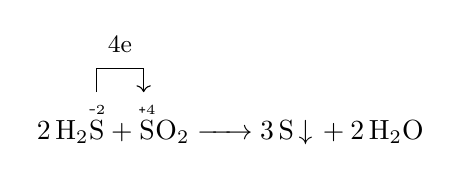
\begin{tikzpicture}
            \node at(0,0) {\ce{2H2$\LiValence{-}{2}{S}$ + $\LiValence{+}{4}{S}$O2 -> 3S v + 2H2O}};
            \LiDrawContainer[->]{(-1.7,0.4)}{(-1.1,0.4)}{0.3}{0.3}{\small \si{4e}};
        \end{tikzpicture}
    \end{center}
    单线桥法需要标注反应物一侧,发生价态变化的元素的化合价。\\[3mm]
    单线桥法的箭头,应当由还原剂中化合价升高的元素,指向氧化剂中化合价降低的元素。

\subsubsection{双线桥法}
    双线桥法也称为长线桥法。\\[3mm]
    双线桥法的第一条线的画法,箭头由还原剂指向氧化产物,并标注“失去”和电子转移数目。\\[3mm]
    双线桥法的第二条线的画法,箭头由氧化剂指向还原产物,并标注“得到”和电子转移数目。\\[3mm]
    双线桥法的例子:
    \begin{center}
        \begin{tikzpicture}
            \node at(0,0) {\ce{2H2$\LiValence{-}{2}{S}$ + $\LiValence{+}{4}{S}$O2 -> 3$\LiValence{}{0}{S}$ v + 2H2O}};
            \LiDrawContainer[->]{(-1.7,+0.4)}{(0.75,+0.4)}{+0.3}{+0.3}{\small 失去~\si{4e}};
            \LiDrawContainer[->]{(-1.1,-0.4)}{(0.75,-0.4)}{-0.3}{-0.3}{\small 得到~\si{4e}};
        \end{tikzpicture}
    \end{center}
    双线桥法需要标注反应式的两侧,发生价态变化的元素的化合价。\\[3mm]
    双线桥法的第一条箭头,应当由还原剂中化合价升高的元素,指向氧化产物中的对应元素。\\[3mm]
    双线桥法的第二条箭头,应当由氧化剂中化合价降低的元素,指向还原产物中的对应元素。

\newpage

\subsection{氧化还原反应的规律}
    氧化还原反应的规律有三条:歧化反应规律,归中反应规律,价态互不换位原则。

\subsubsection{歧化反应规律}
    歧化反应:同一物质的分子中,同一价态的同种元素之间,发生的氧化还原反应。\\[3mm]
    歧化反应的规律为:
    \begin{center}
        \ce{\text{\small 中间价态} -> \text{\small 高价态} + \text{\small 低价态}}\\[3mm]
    \end{center}
    歧化反应的例子:\vspace{-10pt}
    \begin{center}
        \begin{tikzpicture}
            \node at(0,0) {\ce{$\LiValence{}{0}{Cl}$2 + 2NaOH -> Na$\LiValence{-}{1}{Cl}$ + Na$\LiValence{+}{1}{Cl}$O + H2O}};
            \LiDrawContainer[->]{(-3.0,+0.4)}{(1.6,+0.4)}{+0.3}{+0.3}{\small 失去~\si{1e}};
            \LiDrawContainer[->]{(-3.0,-0.4)}{(0.5,-0.4)}{-0.3}{-0.3}{\small 得到~\si{1e}};
        \end{tikzpicture}
    \end{center}
    歧化反应的例子:\vspace{-10pt}
    \begin{center}
        \begin{tikzpicture}
            \node at(0,0) {\ce{3$\LiValence{}{0}{Cl}$2 + 6NaOH ->T[加热] 5Na$\LiValence{-}{1}{Cl}$ + Na$\LiValence{+}{5}{Cl}$O3 + H2O}};
            \LiDrawContainer[->]{(-3.0,+0.4)}{(1.8,+0.4)}{+0.3}{+0.3}{\small 失去~\si{5e}};
            \LiDrawContainer[->]{(-3.0,-0.4)}{(0.6,-0.4)}{-0.3}{-0.3}{\small 得到~\si{1e}};
        \end{tikzpicture}
    \end{center}\vspace{-15pt}

\subsubsection{归中反应规律}
    归中反应:不同物质的分子中,不同价态的同种元素之间,发生的氧化还原反应。\\[3mm]
    归中反应的规律为:
    \begin{center}
        \ce{\text{\small 高价态} + \text{\small 低价态} -> \text{\small 中间价态}}\\[6mm]
    \end{center}
    归中反应的例子:\vspace{-10pt}
    \begin{center}
        \begin{tikzpicture}
            \node at(0,0) {\ce{2H2$\LiValence{-}{2}{S}$ + $\LiValence{+}{4}{S}$O2 -> 3$\LiValence{}{0}{S}$ v + 2H2O}};
            \LiDrawContainer[->]{(-1.7,+0.4)}{(0.75,+0.4)}{+0.3}{+0.3}{\small 失去~\si{4e}};
            \LiDrawContainer[->]{(-1.1,-0.4)}{(0.75,-0.4)}{-0.3}{-0.3}{\small 得到~\si{4e}};
        \end{tikzpicture}
    \end{center}\vspace{-15pt}

\subsubsection{价态互不换位原则}
    价态互不换位原则:同种元素的相邻价态的物质之间,不发生氧化还原反应。\\[3mm]
    如二氧化硫\ce{$\LiValence{+}{4}{S}$O2}具有还原性,而浓硫酸\ce{H2$\LiValence{+}{6}{S}$O4}具有氧化性,但两者中硫的价态相邻故不反应。

\newpage

\subsection{氧化性和还原性强弱的判断}
    金属的活动性顺序表:
    \begin{table}[h]
        \begin{center}
            \begin{tabular}{p{60pt}|p{130pt}|p{140pt}}
                \hline
                金属名称&金属单质(还原性减弱)&金属阳离子(氧化性增强)\\ \hline
                钾&\ce{K}&\ce{K^{+}}\\ \hline
                钙&\ce{Ca}&\ce{Ca^{2+}}\\ \hline
                钠&\ce{Na}&\ce{Na^{+}}\\ \hline
                镁&\ce{Mg}&\ce{Mg^{2+}}\\ \hline
                铝&\ce{Al}&\ce{Al^{3+}}\\ \hline
                锌&\ce{Zn}&\ce{Zn^{2+}}\\ \hline
                铁&\ce{Fe}&\ce{Fe^{2+}}\\ \hline
                锡&\ce{Sn}&\ce{Sn^{2+}}\\ \hline
                铅&\ce{Pb}&\ce{Pb^{2+}}\\ \hline
                氢&\ce{H}&\ce{H^{+}}\\ \hline
                铜&\ce{Cu}&\ce{Cu^{2+}}\\ \hline
                汞&\ce{Hg}&\ce{Hg^{2+}}\\ \hline
                银&\ce{Ag}&\ce{Ag^{+}}\\ \hline
                铂&\ce{Pt}&\ce{Pt^{2+}}\\ \hline
                金&\ce{Au}&\ce{Au^{2+}}\\ \hline
            \end{tabular}
            \caption{金属活动性顺序表}
        \end{center}
    \end{table}\\
    非金属的活动性顺序表:
    \begin{table}[h]
        \begin{center}
            \begin{tabular}{p{60pt}|p{130pt}|p{140pt}}
                \hline
                非金属名称&非金属单质(氧化性减弱)&非金属阴离子(还原性增强)\\ \hline
                氟&\ce{F}&\ce{F^{+}}\\ \hline
                氯&\ce{Cl}&\ce{Cl^{+}}\\ \hline
                溴&\ce{Br}&\ce{Br^{+}}\\ \hline
                碘&\ce{I}&\ce{I^{+}}\\ \hline
                硫&\ce{S}&\ce{S^{2+}}\\ \hline
            \end{tabular}
            \caption{非金属活动性顺序表}
        \end{center}
    \end{table}\\
    金属的单质的还原性,随着活动性顺序表从上至下逐渐减弱。\\[3mm]
    金属阴离子的氧化性,随着活动性顺序表从上至下逐渐增强。\\[3mm]
    非金属的单质的还原性,随着活动性顺序表从上至下逐渐减弱。\\[3mm]
    非金属阳离子的氧化性,随着活动性顺序表从上至下逐渐增强。

\newpage

    同一主族的元素从下到上,对应单质的氧化性逐渐增强,对应阴离子的还原性逐渐减弱。\\[3mm]
    例如氧化性:\ce{I2 $<$ Br2 $<$ Cl2 $<$ F2}。\\[3mm]
    例如还原性:\ce{I- $>$ Br- $>$ Cl- $>$ F-}。\\[6mm]
    同一主族的元素从上到下,对应单质的还原性逐渐增强,对应阳离子的氧化性逐渐减弱。\\[3mm]
    例如还原性:\ce{Li $<$ Na $<$ K $<$ Rb $<$ Cs}。\\[3mm]
    例如氧化性:\ce{Li+ $>$ Na+ $>$ K+ $>$ Rb+ $>$ Cs+}。\\[6mm]
    同一周期的元素从左至右,对应单质的氧化性逐渐增强,对应阴离子的还原性逐渐减弱。\\[3mm]
    例如氧化性:\ce{N2 $<$ O2 $<$ F2}\\[3mm]
    例如还原性:\ce{N^{3-} $>$ O^{2-} $>$ F^{-}}\\[6mm]
    同一周期的元素从右至左,对应单质的还原性逐渐增强,对应阳离子的氧化性逐渐减弱。\\[3mm]
    例如还原性:\ce{Al $<$ Mg $<$ Na}\\[3mm]
    例如氧化性:\ce{Al^{3+} $>$ Mg^{2+} $>$ Na^{+}}\\[6mm]
    变价元素位于最高价态时,有最强的氧化性,无还原性。\\[3mm]
    变价元素位于最低价态时,有最强的还原性,无氧化性。\\[3mm]
    变价元素位于中间价态时,兼有氧化性和还原性,价态越高氧化性越强,价态越低还原性越强。\\[6mm]
    1.浓度越大,对应物质的氧化性越强:
    \begin{center}
        \begin{tabular}{rl}
            &\ce{4H$\LiValence{+}{5}{N}$O3\text{(稀)} + 3Cu -> 3Cu(NO3)2 + 2$\LiValence{-}{2}{N}$O ^ + 4H2O}\\[3mm]
            &\ce{4H$\LiValence{+}{5}{N}$O3\text{(浓)} + Cu ->T[加热] Cu(NO3)2 + 2$\LiValence{-}{4}{N}$O2 ^ + 2H2O}            
        \end{tabular}
    \end{center}\vspace{5pt}
    由此可见氧化性:浓硝酸$>$稀硝酸。\\[8mm]
    2.酸性越强,对应物质的氧化性越强:
    \begin{center}
        \begin{tabular}{rl}
            &\ce{2K\LiValence{+}{7}{Mn}O4 + 2NaOH + Na2SO3 -> 2Na2\LiValence{+}{6}{Mn}O4 + K2SO4 + H2O}\\[3mm]
            &\ce{2K\LiValence{+}{7}{Mn}O4 + H2O + 3Na2SO3 -> 2\LiValence{+}{4}{Mn}O2 + KOH + 3Na2SO4}\\[3mm]
            &\ce{2K\LiValence{+}{7}{Mn}O4 + 3H2SO4 + 5Na2SO3 -> 2\LiValence{+}{2}{Mn}SO4 + K2SO4 + 5NaSO4 + 3H2O}
        \end{tabular}
    \end{center}\vspace{5pt}
    由此可见氧化性:酸性高锰酸钾$>$中性高锰酸钾$>$碱性高锰酸钾。

\newpage

    3.条件相同的情况下,氧化反应越易进行,氧化性越强:
    \begin{center}
        \ce{2K$\LiValence{+}{7}{Mn}$O4 + 16HCl\text{(浓)} -> 2$\LiValence{+}{2}{Mn}$Cl2 + 2KCl + 8H2O + 5Cl2 ^}\\[3mm]
        \ce{$\LiValence{+}{4}{Mn}$O2 + 4HCl\text{(浓)} ->T[加热] $\LiValence{+}{2}{Mn}$Cl2 + 2H2O + Cl2 ^}\\[3mm]
    \end{center}
    由此可见氧化性:\ce{KMnO4 $>$ MNO2}。\\[12mm]
    4.氧化的程度越彻底,氧化剂的氧化性越强:\vspace{5pt}
    \begin{center}
        \ce{$\LiValence{}{0}{Fe}$ + S ->T[加热] $\LiValence{+}{2}{Fe}$S}\\[3mm]
        \ce{2$\LiValence{}{0}{Fe}$ + 3Cl2 ->T[点燃] 2$\LiValence{+}{3}{Fe}$Cl3}\\[3mm]
    \end{center}
    由此可见氧化性:\ce{Cl2 $>$ S}。\\[3mm]
    因为硫单质和铁反应,只能使其被氧化至$+2$价。\\[3mm]
    同时氯单质和铁反应,却能使其被氧化至$+3$价。\\[12mm]
    5.还原的程度越彻底,还原剂的还原性越强:\vspace{5pt}
    \begin{center}
        \ce{H2$\LiValence{+}{6}{S}$O4\text{(浓)} + 2HBr -> $\LiValence{+}{4}{S}$O2 ^ + Br2 + 2H2O}\\[3mm]
        \ce{H2$\LiValence{+}{6}{S}$O4\text{(浓)} + 8HI -> H2$\LiValence{-}{2}{S}$ ^ + 4I2 + 4H2O}\\[3mm]
    \end{center}
    由此可见还原性:\ce{HBr $>$ HI}。\\[3mm]
    因为溴化氢和浓硫酸反应,只能使其被还原至$+4$价。\\[3mm]
    同时碘化氢和浓硫酸反应,却能使其被还原至$-2$价。\\[12mm]
    6.由氧化还原反应的通式:
    \begin{center}
        \ce{\text{\small 氧化剂} + \text{\small 还原剂} -> \text{\small 氧化产物} + \text{\small 还原产物}}\\[6mm]
    \end{center}
    氧化剂的氧化性强于氧化产物,氧化剂的氧化性强于还原剂。\\[3mm]
    还原剂的还原性强于还原产物,还原剂的还原性强于氧化剂。

\newpage

\section{卤族元素}

\subsection{氯气}
    氯气,黄绿色刺激性气味的气体,密度$3.21$\si{g/L},熔点$-101$\si{\degreeCelsius},沸点$-35$\si{\degreeCelsius}。\\[3mm]
    氯气可溶于水,常温下$1$体积的水可以溶解$2$体积的氯气。

\subsubsection{氯气和金属的反应}
    氯气可以和钠反应,生成白色固体(氯化钠):
    \begin{center}
        \ce{2Na + Cl2 ->T[点燃] 2NaCl}\\[6mm]
    \end{center}
    氯气可以和铁反应,生成棕褐色的烟(氯化铁):
    \begin{center}
        \ce{2Fe + 3Cl2 ->T[点燃] 2FeCl3}\\[6mm]
    \end{center}
    氯气可以和铜反应,生成棕黄色的烟(氯化铜):
    \begin{center}
        \ce{Cu + 2Cl2 ->T[点燃] CuCl2}\\[6mm]
    \end{center}
    氯气的氧化性较强,可以在点燃的条件下与绝大多数金属反应,且可以反应至最高价态。

\subsubsection{氯气和非金属的反应}
    氯气和氢气可以在点燃的条件下安静的燃烧,产生白雾:
    \begin{center}
        \ce{H2 + Cl2 ->T[点燃] 2HCl}\\[6mm]
    \end{center}
    氯气和氢气可以在光照的条件下剧烈的爆炸,产生白雾:
    \begin{center}
        \ce{H2 + Cl2 ->T[光照] 2HCl}\\[6mm]
    \end{center}
    其中产生的白雾为氯化氢和水结合的产物。\\[3mm]
    在以点燃为条件的反应中,会观察到苍白色火焰。\\[3mm]
    在以光照为条件的反应中,通常会使用镁带燃烧产生的耀眼的白光作为光源。\\[8mm]
    氯气和磷在点燃的条件下会燃烧,产生白色烟雾:
    \begin{center}
        \ce{2P + 3Cl2 ->T[点燃] 2PCl3}\\[3mm]
        \ce{2P + 5Cl2 ->T[点燃] 2PCl5}\\[6mm]
    \end{center}
    其中产生的白色烟雾由液体状态的三氯化磷和固体状态的五氯化磷混合而成。

\newpage

\subsubsection{氯气的实验室制法}
    氯气可以用浓盐酸和二氧化锰制取:
    \begin{center}
        \ce{MnO2 + HCl\text{(浓)} ->T[加热] MnCl2 + Cl2 ^ + 2H2O}\\[6mm]
    \end{center}
    氯气制取时的具体步骤如下:在烧瓶中加入少量的二氧化锰粉末,用分液漏斗缓缓加入浓盐酸,
    稍稍加热提高反应速度,首先通过饱和的食盐水,使得氯化氢被吸收,同时保证氯气不被吸收,
    然后通过浓硫酸,使得水被吸收,用向上排空气法收集氯气,用氢氧化钠处理尾气。

\subsubsection{氯气和水的反应}
    氯气可以溶于水,氯气溶于水的产物称为氯水。\\[3mm]
    氯气溶于水的同时也可以和水发生反应,生成盐酸和次氯酸:
    \begin{center}
        \ce{Cl2 + H2O <=> HCl + HClO}\\[6mm]
    \end{center}
    氯气和水反应得到的次氯酸在光照下会分解,生成盐酸和氧气:
    \begin{center}
        \ce{2HClO ->T[光照] 2HCl + O2 ^}\\[6mm]
    \end{center}
    因此氯水旧置后,随着次氯酸的分解,促进可逆反应不断正向进行,最终全部转化为氯化氢。\\[6mm]
    准备两个集气瓶,一个装有湿色布,一个装有干色布,通入氯气。\\[3mm]
    实验可以观察到,干色布无褪色现象,说明氯气无漂白性。\\[3mm]
    实验可以观察到,湿色布有褪色现象,说明氯水有漂白性。\\[3mm]
    两者对比可知,氯水中的次氯酸具有漂白性。\\[6mm]
    次氯酸具有漂白性,常利用其可以使有机染料褪色的特性,作为漂白剂。\\[3mm]
    次氯酸具有强氧化性,常利用其可以杀灭病菌的特性,作为自来水的消毒剂。

\newpage

\subsubsection{氯气和碱的反应}
    氯气可以和氢氧化钠反应,生成氯化钠和次氯酸钠:
    \begin{center}
        \ce{Cl2 + 2NaOH -> NaCl + NaClO + H2O}\\[6mm]
    \end{center}
    氯气可以和氢氧化钙反应,生成氯化钙和次氯酸钙:
    \begin{center}
        \ce{2Cl2 + 2Ca(OH)2 -> CaCl2 + Ca(ClO)2 + 2H2O}\\[6mm]
    \end{center}
    漂白粉指的就是氯气和氢氧化钠反应得到的混合物,其有效成分是次氯酸钠。\\[9mm]
    次氯酸钠可以和盐酸反应,生成氯化钠和次氯酸:
    \begin{center}
        \ce{NaClO + HCl -> NaCl + HClO}\\[6mm]
    \end{center}
    次氯酸钙可以和盐酸反应,生成氯化钙和次氯酸:
    \begin{center}
        \ce{Ca(ClO)2 + 2HCl -> CaCl2 + 2HClO}\\[6mm]
    \end{center}
    次氯酸钠可以和二氧化碳和水反应,生成碳酸氢钠和次氯酸:
    \begin{center}
        \ce{NaClO + CO2 + H2O -> NaHCO3 + HClO}\\[6mm]
    \end{center}
    次氯酸钙可以和二氧化碳和水反应,生成碳酸氢钙和次氯酸:
    \begin{center}
        \ce{Ca(ClO)2 + 2CO2 + 2H2O -> Ca(HCO3)2 + 2HClO}\\[6mm]
    \end{center}
    漂白粉使用时,既可以与稀酸反应,也可以与空气中的二氧化碳和水蒸气反应。\\[3mm]
    漂白粉是固体且较为稳定,也可以反应生成次氯酸,而相较于次氯酸又便于储存携带。

\newpage

\subsection{氯化氢}
    氯化氢,无色刺激性气味的气体,密度$1.48$\si{kg/m^3},熔点$-144$\si{\degreeCelsius},沸点$-85$\si{\degreeCelsius}。\\[3mm]
    氯化氢易溶于水,常温下$1$体积的水可以溶解$500$体积的氯化氢。\\[3mm]
    氯化氢溶于水的产物称为盐酸。

\subsubsection{氯化氢的实验室制法}
    氯化氢可以用浓硫酸和氯化钠制取:
    \begin{center}
        \ce{NaCl + H2SO4\text{(浓)} ->T[微热] NaHSO4 + HCl ^}\\[3mm]
        \ce{2NaCl + H2SO4\text{(浓)} ->T[强热] Na2SO4 + 2HCl ^}\\[6mm]
    \end{center}
    氯化氢的制取反应中,微热时生成硫酸氢钠,强热时生成硫酸钠。\\[3mm]
    氯化氢制取时的具体步骤如下:在烧瓶中加入少量的氯化钠粉末,用分液漏斗缓缓加入浓硫酸,
    用酒精灯加热提高反应速度,用向上排空气法收集,用水处理尾气。\\

\subsection{盐酸}
    盐酸,无色腐蚀性液体,密度$1.18$\si{g/cm^3},熔点$-26$\si{\degreeCelsius},沸点$48$\si{\degreeCelsius}。\\[3mm]
    盐酸可以分为稀盐酸和浓盐酸,稀盐酸为低沸点的非氧化性酸,浓盐酸为低沸点的非氧化性酸。\\[3mm]
    盐酸是一元强酸,具有酸的通性。\\[6mm]
    浓盐酸的质量分数为$\omega=37\%$。\\[3mm]
    浓盐酸中的氯化氢常会挥发与空气中的水蒸气结合形成白雾。\\[3mm]
    盐酸为无色液体,但工业盐酸由于含有铁等杂质而显黄色。\\[6mm]
    盐酸的电离方程式:
    \begin{center}
        \ce{HCl -> H+ + Cl-}\\[6mm]
    \end{center}
    盐酸可以使紫色石蕊试剂由紫色变为红色。\\[3mm]
    盐酸可以使甲基橙指示剂由橙色变为红色。

\newpage

\subsubsection{盐酸和金属的反应}
    盐酸可以和活泼金属反应:
    \begin{center}
        \ce{2HCl + Fe -> FeCl2 + H2 ^}\\[3mm]
        \ce{6HCl + 3Al -> 2AlCl3 + 3H2 ^}\\[6mm]
    \end{center}\vspace{5pt}

\subsubsection{盐酸和氧化物的反应}
    盐酸可以和碱性氧化物反应:
    \begin{center}
        \ce{2HCl + CaO -> CaCl2 + H2O}\\[3mm]
        \ce{2HCl + CuO -> CuCl2 + H2O}\\[6mm]
    \end{center}
    盐酸可以和两性氧化物反应:
    \begin{center}
        \ce{6HCl + Al2O3 -> 2AlCl3 + 3H2O}
    \end{center}\vspace{5pt}

\subsubsection{盐酸和碱的反应}
    盐酸可以和强碱反应:
    \begin{center}
        \ce{HCl + NaOH -> NaCl + H2O}\\[3mm]
        \ce{HCl + KOH -> KCl + H2O}\\[6mm]
    \end{center}
    盐酸可以和弱碱反应:
    \begin{center}
        \ce{Cu(OH)2 + 2HCl -> CuCl2 + H2O}
    \end{center}\vspace{5pt}

\subsubsection{盐酸和盐的反应}
    盐酸可以和部分盐反应:
    \begin{center}
        \ce{2HCl + CaCO3 -> CaCl2 + H2O + CO2 ^}\\[3mm]
        \ce{2HCl + Na2CO3 -> 2NaCl + H2O + CO2 ^}\\[6mm]
    \end{center}
    盐酸可以和硝酸银反应产生白色沉淀:
    \begin{center}
        \ce{HCl + AgNO3 -> AgCl v + HNO3}\\[6mm]
    \end{center}
    氯化银是一种白色沉淀,不溶于水,不溶于硝酸,溶于氨水,该反应可以用于检验氯离子。

\newpage

\subsection{卤族元素}
    卤族元素包含五种元素:氟(\ce{F}),氯(\ce{Cl}),溴(\ce{Br}),碘(\ce{I}),砹(\ce{At})。\\[3mm]
    卤族元素位于元素周期表中的\rnum{7}A族。\\[3mm]
    卤族元素的原子结构如下:\vspace{5pt}
    \begin{table}[h]
        \begin{center}
            \begin{tabular}{p{50pt}|p{75pt}|p{55pt}|p{70pt}|p{100pt}}
                \hline
                元素名称&原子半径&原子序数&电子层排布&主要化合价\\ \hline
                氟(\ce{F})&$0.64\times 10^{-10}$\si{m}&$9$&$2$-$7$&$-1$~~$+1$~~$+3$~~$+5$~~$+7$\\ \hline
                氯(\ce{Cl})&$0.99\times 10^{-10}$\si{m}&$17$&$2$-$8$-$7$&$-1$~~$+1$~~$+3$~~$+5$~~$+7$\\ \hline
                溴(\ce{Br})&$1.14\times 10^{-10}$\si{m}&$35$&$2$-$8$-$18$-$7$&$-1$~~$+1$~~$+3$~~$+5$~~$+7$\\ \hline
                碘(\ce{I})&$1.33\times 10^{-10}$\si{m}&$53$&$2$-$8$-$18$-$18$-$7$&$-1$~~$+1$~~$+3$~~$+5$~~$+7$\\ \hline
                砹(\ce{At})&$1.45\times 10^{-10}$\si{m}&$85$&$2$-$8$-$18$-$32$-$18$-$7$&$-1$~~$+1$~~$+3$~~$+5$~~$+7$\\ \hline
            \end{tabular}
            \caption{卤族元素的原子结构}
        \end{center}
    \end{table}\\
    卤族元素的电子亚层如下:\vspace{5pt}
    \begin{table}[h]
        \begin{center}
            \begin{tabular}{p{50pt}|p{30pt}|p{40pt}|p{55pt}|p{65pt}|p{50pt}|p{35pt}}
                \hline
                元素名称&K层&L层&M层&N层&O层&P层\\ \hline
                氟(\ce{F})&\si{1s^2}&\si{2s^2 2p^5}&&&&\\ \hline
                氯(\ce{Cl})&\si{1s^2}&\si{2s^2 2p^6}&\si{3s^2 3p^5}&&&\\ \hline
                溴(\ce{Br})&\si{1s^2}&\si{2s^2 2p^6}&\si{3s^2 3p^6 3d^{10}}&\si{4s^2 4p^5}&&\\ \hline
                碘(\ce{I})&\si{1s^2}&\si{2s^2 2p^6}&\si{3s^2 3p^6 3d^{10}}&\si{4s^2 4p^6 4d^{10}}&\si{5s^2 5p^{5}}&\\ \hline
                砹(\ce{At})&\si{1s^2}&\si{2s^2 2p^6}&\si{3s^2 3p^6 3d^{10}}&\si{4s^2 4p^6 4d^{10} 4f^{14}}&\si{5s^2 5p^{6} 5d^{10}}&\si{6s^2 6p^{5}}\\ \hline
            \end{tabular}
            \caption{卤族元素的电子亚层}
        \end{center}
    \end{table}\\
    卤族元素的单质性质如下:\vspace{5pt}
    \begin{table}[h]
        \begin{center}
            \begin{tabular}{p{50pt}|p{85pt}|p{75pt}|p{70pt}|p{70pt}}
                \hline
                单质类型&颜色和状态&密度&熔点&沸点\\ \hline
                氟&淡黄绿色气体&$1.69$\si{g/L}&$-220$\si{\degreeCelsius}&$-188$\si{\degreeCelsius}\\ \hline
                氯&黄绿色气体&$3.21$\si{g/L}&$-101$\si{\degreeCelsius}&$-35$\si{\degreeCelsius}\\ \hline
                溴&棕红色液体&$3.20$\si{g/cm^3}&$-7$\si{\degreeCelsius}&$+59$\si{\degreeCelsius}\\ \hline
                碘&紫黑色固体&$4.93$\si{g/cm^3}&$+114$\si{\degreeCelsius}&$+184$\si{\degreeCelsius}\\ \hline
            \end{tabular}
        \end{center}
    \end{table}\\
    卤族元素最外层均为七个电子,但电子层数有所不同。\\[3mm]
    卤族元素随着原子序数的增加,熔沸点逐渐升高,颜色逐渐加深。

\newpage

\subsubsection{卤素和金属的反应}
    氯可以和钠在燃烧的条件下反应,生成白色固体:
    \begin{center}
        \ce{Cl2 + 2Na ->T[点燃] 2NaCl}\\[4mm]
    \end{center}
    碘可以和锌在有水的条件下反应,生成紫色蒸汽:
    \begin{center}
        \ce{I2 + Zn ->T[水] ZnI2}\\[4mm]
    \end{center}
    该反应产生的紫色蒸汽,是由于反应大量放热,导致碘升华为碘蒸汽。\\[3mm]
    卤素性质均是较为活泼的非金属,因此都能和绝大多数金属发生反应。\\[3mm]
    卤素中的氟尤其活泼,甚至可以和稀有气体中的氙(\ce{Xe})和氪(\ce{Kr})反应生成对应氟化物。\vspace{5pt}

\subsubsection{卤素和非金属的反应}
    氟和氢气可以在阴暗处剧烈反应,发生爆炸:
    \begin{center}
        \ce{F2 + H2 -> 2HF}\\[4mm]
    \end{center}
    氯和氢气可以在光照下剧烈反应,发生爆炸:
    \begin{center}
        \ce{Cl2 + H2 ->T[光照] 2HCl}\\[4mm]
    \end{center}
    溴和氢气需要在加热的条件下缓慢反应:
    \begin{center}
        \ce{Br2 + H2 ->T[加热] 2HBr}\\[4mm]
    \end{center}
    碘和氢气需要在高温的条件下缓慢反应:
    \begin{center}
        \ce{I2 + H2 <=>T[高温] 2HBr}\\[4mm]
    \end{center}
    卤素单质和氢气反应放出的热量分别为(以$1$\si{mol}卤素单质计):\vspace{5pt}
    \begin{table}[h]
        \begin{center}
            \begin{tabular}{p{120pt}|p{120pt}}
                \hline
                与氢气反应的卤素单质&所放出或吸收的热量\\ \hline
                氟(\ce{F2})&$+572.2$\si{kJ}\\ \hline
                氯(\ce{Cl2})&$+92.3$\si{kJ}\\ \hline
                溴(\ce{Br2})&$+36.4$\si{kJ}\\ \hline
                碘(\ce{I2})&$-51.9$\si{kJ}\\ \hline
            \end{tabular}
        \end{center}
    \end{table}\\
    卤素单质的活泼性随原子序数的增大而逐渐减小,即氟单质较为活泼,而碘单质较为不活泼。\\[3mm]
    卤化氢的稳定程度随原子序数的增大而逐渐减小,即氟化氢较为稳定,而碘化氢较为不稳定。

\newpage

\subsubsection{卤素和盐的反应}
    氯可以和溴化钠反应,生成氯化钠和溴:
    \begin{center}
        \ce{Cl2 + NaBr -> 2NaCl + Br2}\\[6mm]
    \end{center}
    氯可以和碘化钾反应,生成氯化钾和碘:
    \begin{center}
        \ce{Cl2 + KI -> 2KCl + I2}\\[6mm]
    \end{center}
    溴可以和碘化钾反应,生成溴化钾和碘:
    \begin{center}
        \ce{Br2 + KI -> 2KBr + I2}\\[6mm]
    \end{center}
    由此可知,氯可以从溴盐中置换出溴单质。\\[3mm]
    由此可知,氯可以从碘盐中置换出碘单质。\\[3mm]
    由此可知,溴可以从碘盐中置换出碘单质。\\[3mm]
    因此,氯的活动性强于溴,溴的活动性强于碘。\\[8mm]
    卤素单质可以被有机溶剂从水中萃取,因此上述反应中常加入有机溶剂判断生成的单质。\\[3mm]
    卤素单质萃取时常用的有机溶剂包含:苯(\ce{C6H6}),四氯化碳(\ce{CCl4}),汽油。\\[3mm]
    卤素单质溶于有机溶剂的颜色如下:\vspace{5pt}
    \begin{table}[h]
        \begin{center}
            \begin{tabular}{p{80pt}|p{120pt}|p{120pt}}
                \hline
                卤素单质&稀的四氯化碳溶液颜色&浓的四氯化碳溶液颜色\\ \hline
                氯(\ce{Cl2})&黄绿色&黄绿色\\ \hline
                溴(\ce{Br2})&橙黄色&橙红色\\ \hline
                碘(\ce{I2})&浅紫色&紫红色\\ \hline
            \end{tabular}
            \caption{卤素单质的四氯化碳溶液的颜色}
        \end{center}
    \end{table}\\
    此外由于氯气和碘化钾反应会得到碘单质:
    \begin{center}
        \ce{Cl2 + KI -> 2KCl + I2}\\[6mm]
    \end{center}
    因此氯气常用淀粉碘化钾试纸检验,会观察到试纸由白色变为蓝色。\\[3mm]
    因为氯气和碘化钾反应得到的碘单质会使淀粉变蓝。\\[8mm]

\newpage

\subsubsection{卤素和水的反应}
    氟和水可以剧烈反应,生成氢氟酸和氧气:
    \begin{center}
        \ce{2F2 + 2H2O -> 4HF + O2}\\[6mm]
    \end{center}
    氯和水可以进行反应,生成氢氯酸和次氯酸:
    \begin{center}
        \ce{Cl2 + H2O <=> HCl + HClO}\\[6mm]
    \end{center}
    溴和水反应较为缓慢,生成氢溴酸和次溴酸:
    \begin{center}
        \ce{Br2 + H2O <=> HBr + HBrO}\\[6mm]
    \end{center}
    碘和水反应非常缓慢,生成氢碘酸和次碘酸:
    \begin{center}
        \ce{I2 + H2O <=> HI + HIO}\\[6mm]
    \end{center}
    卤素单质除了和水反应,还可以溶于水。\\[3mm]
    卤素单质溶于水的颜色如下:\vspace{5pt}
    \begin{table}[h]
        \begin{center}
            \begin{tabular}{p{80pt}|p{100pt}|p{100pt}}
                \hline
                卤素单质&稀的水溶液颜色&浓的水溶液颜色\\ \hline
                氯(\ce{Cl2})&黄绿色&黄绿色\\ \hline
                溴(\ce{Br2})&黄色&橙黄色\\ \hline
                碘(\ce{I2})&黄色&棕黄色\\ \hline
            \end{tabular}
            \caption{卤素单质的水溶液的颜色}
        \end{center}
    \end{table}\\
    次氯酸不稳定,会自发的分解为氢氯酸和氧气:
    \begin{center}
        \ce{2HClO -> 2HCl + O2 ^}\\[6mm]
    \end{center}
    次溴酸不稳定,会自发的分解为氢溴酸和氧气:
    \begin{center}
        \ce{2HBrO -> 2HBr + O2 ^}\\[6mm]
    \end{center}
    次碘酸不稳定,会自发的分解为氢碘酸和氧气:
    \begin{center}
        \ce{2HBrO -> 2HI + O2 ^}\\[6mm]
    \end{center}
    次氯酸,次溴酸,次碘酸,三者均为弱酸,具有强氧化性。\\[3mm]
    氢氯酸,氢溴酸,氢碘酸,三者均为强酸,具有还原性。\\[3mm]
    氢氟酸在氢卤酸中是一个特殊的例外,其为弱酸。

\newpage

\subsubsection{卤素和碱的反应}
    氯和氢氧化钠反应,常温条件生成次氯酸钠和氯化钠:
    \begin{center}
        \ce{Cl2 + 2NaOH -> NaCl + NaClO + H2O}\\[6mm]
    \end{center}
    溴和氢氧化钠反应,常温条件生成次溴酸钠和溴化钠:
    \begin{center}
        \ce{Br2 + 2NaOH -> NaBr + NaBrO + H2O}\\[6mm]
    \end{center}
    碘和氢氧化钠反应,常温条件生成次碘酸钠和碘化钠:
    \begin{center}
        \ce{I2 + 2NaOH -> NaI + NaIO + H2O}\\[6mm]
    \end{center}
    氯和氢氧化钠反应,加热条件生成氯酸钠和氯化钠:
    \begin{center}
        \ce{3Cl2 + 6NaOH ->T[加热] 5NaCl + NaClO3 + H2O}\\[6mm]
    \end{center}
    溴和氢氧化钠反应,加热条件生成溴酸钠和溴化钠:
    \begin{center}
        \ce{3Br2 + 6NaOH ->T[加热] 5NaBr + NaBrO3 + H2O}\\[6mm]
    \end{center}
    碘和氢氧化钠反应,加热条件生成碘酸钠和碘化钠:
    \begin{center}
        \ce{3I2 + 6NaOH ->T[加热] 5NaI + NaIO3 + H2O}\\[6mm]
    \end{center}
    在常温条件下反应时,一份卤原子被还原至$-1$价,一份卤原子被氧化至$+1$价。\\[3mm]
    在加热条件下反应时,五份卤原子被还原至$-1$价,一份卤原子被氧化至$+5$价。

\newpage

\subsubsection{卤化银的性质}
    氯化钠和硝酸银反应,生成氯化银沉淀:
    \begin{center}
        \ce{NaCl + AgNO3 -> NaNO3 + AgCl v}\\[6mm]
    \end{center}
    溴化钠和硝酸银反应,生成溴化银沉淀:
    \begin{center}
        \ce{NaBr + AgNO3 -> NaNO3 + AgBr v}\\[6mm]
    \end{center}
    碘化钾和硝酸银反应,生成碘化银沉淀:
    \begin{center}
        \ce{KI + AgNO3 -> KNO3 + AgI v}\\[6mm]
    \end{center}
    卤化银的颜色如下:
    \begin{table}[h]
        \begin{center}
            \begin{tabular}{p{100pt}|p{100pt}}
                \hline
                卤化银类型&卤化银颜色\\ \hline
                氯化银(\ce{AgCl})&白色\\ \hline
                溴化银(\ce{AgBr})&淡黄色\\ \hline
                碘化银(\ce{AgI})&黄色\\ \hline
            \end{tabular}
            \caption{卤化银的颜色}
        \end{center}
    \end{table}\\
    溴化银具有感光性,光照下会分解:
    \begin{center}
        \ce{2AgBr ->T[光照] 2Ag + Br2}\\[6mm]
    \end{center}
    碘化银具有感光性,光照下会分解:
    \begin{center}
        \ce{2AgI ->T[光照] 2Ag + I2}\\[6mm]
    \end{center}
    胶片相机中所用的感光胶片,就是由溴化银均匀的涂在胶卷上制成的。

\newpage

\subsubsection{卤化氢的制备}
    氟化钙和浓硫酸反应,生成氟化氢:
    \begin{center}
        \ce{CaF2 + H2SO4\text{(浓)} ->T[加热] CaSO4 + 2HF ^}\\[6mm]
    \end{center}
    氯化钠和浓硫酸反应,生成氯化氢:
    \begin{center}
        \ce{NaCl + H2SO4\text{(浓)} ->T[微热] NaHSO4 + HCl ^}\\[6mm]
    \end{center}
    溴化钠和浓磷酸反应,生成溴化氢:
    \begin{center}
        \ce{NaBr + H3PO4\text{(浓)} ->T[加热] NaH2PO4 + HBr ^}\\[6mm]
    \end{center}
    碘化钠和浓磷酸反应,生成碘化氢:
    \begin{center}
        \ce{NaI + H3PO4\text{(浓)} ->T[加热] NaH2PO4 + HI ^}\\[6mm]
    \end{center}
    以上反应用稀硫酸均不反应,因为此处利用的原理,是高沸点酸制低沸点酸,不是强酸制弱酸,
    虽然稀硫酸是强酸,但是稀硫酸不是高沸点酸,其沸点和水相近,故不发生反应。\\[8mm]
    制取氯化氢时不能加强热,否则会导致温度过高使得浓硫酸溢出:\vspace{5pt}
    \begin{center}
        \ce{NaCl + H2SO4\text{(浓)} ->T[微热] NaHSO4 + HCl ^}\\[3mm]
        \ce{2NaCl + H2SO4\text{(浓)} ->T[强热] Na2SO4 + 2HCl ^}\\[6mm]
    \end{center}
    制取溴化氢时不能使用浓硫酸,因为溴化氢会被浓硫酸氧化:
    \begin{center}
        \ce{2NaBr + 3H2SO4\text{(浓)} ->T[加热] NaHSO4 + SO2 ^ + 2H2O + Br2}\\[6mm]
    \end{center}
    制取碘化氢时不能使用浓硫酸,因为碘化氢会被浓硫酸氧化:
    \begin{center}
        \ce{2NaI + 3H2SO4\text{(浓)} ->T[加热] NaHSO4 + SO2 ^ + 2H2O + I2}\\[6mm]
    \end{center}
    浓硫酸可以用于制取氯化氢,是因为其还原性较弱,无法与浓硫酸反应。\\[3mm]
    浓硫酸不能用于制取溴化氢,是因为其还原性较强,可以与浓硫酸反应。\\[3mm]
    浓硫酸不能用于制取碘化氢,是因为其还原性较强,可以与浓硫酸反应。\\[3mm]
    浓硫酸的氧化性较强,浓磷酸的氧化性较弱,因此选用后者可以避免溴化氢和碘化氢被氧化。

\newpage

\section{氧族元素}

\subsection{硫}
    硫,淡黄色臭味的晶体,密度$2.08$\si{g/cm^3},熔点$113$\si{\degreeCelsius},沸点$445$\si{\degreeCelsius}。\\[3mm]
    硫有多种同素异形体,包括\ce{S2},\ce{S4},\ce{S6},\ce{S8},其中以~\ce{S8}最常见,均可以用~\ce{S}统一表示。\\[3mm]
    硫难溶于水,微溶于酒精,易溶于二硫化碳。

\subsubsection{硫和金属的反应}
    硫可以和铁反应,生成黑色的固体(硫化亚铜):
    \begin{center}
        \ce{2Cu + S ->T[加热] Cu2S}\\[6mm]
    \end{center}
    硫可以和铁反应,生成黑褐色固体(硫化亚铁):
    \begin{center}
        \ce{Fe + S ->T[加热] FeS}\\[6mm]
    \end{center}
    硫可以和铁反应,生成黑色的固体(硫化汞):
    \begin{center}
        \ce{Hg + S ->T[加热] HgS}\\[6mm]
    \end{center}
    硫的氧化性较弱,只能在加热的条件下与绝大多数金属反应,但只能反应至最低价态。\\[3mm]
    硫和汞的反应是一个例外,无需加热且可以氧化至最高价态,这是因为汞是液体易于反应。\\[3mm]
    硫和汞的反应常用于在实验室处收集散落的汞滴,减轻汞蒸气造成的污染。\\[3mm]
    硫和铁的反应统称将硫粉和铁粉混合加热,实验会观察到红热现象。

\subsubsection{硫和非金属的反应}
    硫可以和氢气化合,生成臭鸡蛋气味的气体:
    \begin{center}
        \ce{S + H2 ->T[加热] H2S}\\[6mm]
    \end{center}
    硫可以和氧气燃烧,生成刺激性气味的气体:
    \begin{center}
        \ce{S + O2 ->T[点燃] SO2}\\[6mm]
    \end{center}
    硫在空气中燃烧火焰为淡蓝色。\\[3mm]
    硫在氧气中燃烧火焰为蓝紫色。

\newpage

\subsubsection{硫和酸碱盐的反应}
    硫可以和亚硫酸钠反应,生成硫代硫酸钠:
    \begin{center}
        \ce{S + Na2SO3 -> Na2S2SO3}\\[4mm]
    \end{center}
    硫可以和氧化性的酸反应,生成二氧化硫:
    \begin{center}
        \ce{S + 2H2SO4\text{(浓)} ->T[加热] 3SO2 ^ + 2H2O}\\[4mm]
    \end{center}
    硫可以和热的碱溶液反应,生成硫化物和亚硫酸盐:
    \begin{center}
        \ce{3S + 6KOH ->T[加热] 2K2S + K2SO3 + 3H2O}\\[4mm]
    \end{center}

\subsection{硫化氢}
    硫化氢,无色臭鸡蛋气味的气体,密度$1.54$\si{g/L},熔点$-86$\si{\degreeCelsius},沸点$-60$\si{\degreeCelsius}。\\[3mm]
    硫化氢可溶于水,常温下$1$体积的水可溶解$2.6$体积的硫化氢。\\[3mm]
    硫化氢溶于水的产物称为氢硫酸。

\subsubsection{硫化氢的还原性}
    硫化氢可以被氧气氧化,产生硫:
    \begin{center}
        \ce{2H2S + O2 -> 2S v + 2H2O}\\[4mm]
    \end{center}
    硫化氢可以被氯水氧化,氯水褪色,产生黄色的硫沉淀:
    \begin{center}
        \ce{H2S + Cl2 -> 2HCl + S v}\\[4mm]
    \end{center}
    硫化氢可以被溴水氧化,溴水褪色,产生黄色的硫沉淀:
    \begin{center}
        \ce{H2S + Br2 -> 2HBr + S v}\\[4mm]
    \end{center}
    硫化氢可以被碘水氧化,碘水褪色,产生黄色的硫沉淀:
    \begin{center}
        \ce{H2S + I2 -> 2HI + S v}\\[4mm]
    \end{center}
    硫化氢可以被过量氯水进一步氧化,产生硫酸:
    \begin{center}
        \ce{H2S + 4Cl2 + 4H2O -> H2SO4 + 8HCl}\\[4mm]
    \end{center}
    硫化氢可以被酸性高锰酸钾氧化,产生硫酸根:
    \begin{center}
        \ce{5H2S + 8KMnO4 + 7H2SO4 -> 8MnSO4 + 4K2SO4 + 2H2O}\\[4mm]
    \end{center}
    氢硫酸溶液置于空气中会变得混浊,这是因为硫化氢会被空气中的氧气氧化产生硫沉淀。

\newpage

\subsubsection{硫化氢的实验室制法}
    硫化氢可以用硫化亚铁和稀硫酸制取:
    \begin{center}
        \ce{FeS + H2SO4 -> FeSO4 + H2S ^}\\[6mm]
    \end{center}
    硫化氢可以用硫化亚铁和稀盐酸制取:
    \begin{center}
        \ce{FeS + HCl -> FeCl2 + H2S ^}\\[6mm]
    \end{center}
    硫化氢制取时的具体步骤如下:启普发生器中加入硫化亚铁固体和稀硫酸或稀盐酸,打开活塞,使得反应进行,
    用向上排空气法收集,用氢氧化钠收集尾气。\\

\subsubsection{硫化氢的可燃性}
    硫化氢在氧气充足时燃烧,产生二氧化硫:
    \begin{center}
        \ce{2H2S + 3O2 ->T[点燃] 2SO2 + 2H2O}\\[6mm]
    \end{center}
    硫化氢在氧气不足时燃烧,产生硫单质:
    \begin{center}
        \ce{2H2S + 3O2 ->T[点燃] 2SO2 + 2H2O}\\[6mm]
    \end{center}
    硫化氢和氧气燃烧火焰为蓝色火焰。\\

\subsubsection{硫化氢和盐的反应}
    硫化氢和醋酸铅溶液反应,产生棕黑色的沉淀:
    \begin{center}
        \ce{H2S + PbAc -> 2HAc + PbS v}\\[6mm]
    \end{center}
    硫化氢和硝酸铅溶液反应,产生棕黑色的沉淀:
    \begin{center}
        \ce{H2S + Pb(NO3)2 -> 2HNO3 + PbS v}\\[6mm]
    \end{center}
    硫化氢和硫酸铜溶液反应,产生黑色的沉淀:
    \begin{center}
        \ce{H2S + CuSO4 -> 2H2SO4 + CuS v}\\[6mm]
    \end{center}
    因此硫化氢常用醋酸铅试纸检验,会观察到试纸由白色变为黑色。

\newpage

\subsection{二氧化硫}
    二氧化硫,无色刺激性气味气体,密度$2.93$\si{g/L},熔点$-73$\si{\degreeCelsius},沸点$-10$\si{\degreeCelsius}。\\[3mm]
    二氧化硫易溶于水,常温下$1$体积的水可以溶解$40$体积的二氧化硫。

\subsubsection{二氧化硫的还原性}
    二氧化硫的还原性较强。\\[3mm]
    二氧化硫可以被氧气氧化,产生三氧化硫:
    \begin{center}
        \ce{2SO2 + O2 <=>T[\ce{V2O5}][加热] 2SO3}\\[6mm]
    \end{center}
    二氧化硫可以被氯水氧化,氯水褪色,产生硫酸:
    \begin{center}
        \ce{SO2 + Cl2 + 2H2O -> 2HCl + H2SO4}\\[6mm]
    \end{center}
    二氧化硫可以被溴水氧化,溴水褪色,产生硫酸:
    \begin{center}
        \ce{SO2 + Br2 + 2H2O -> 2HBr + H2SO4}\\[6mm]
    \end{center}
    二氧化硫可以被碘水氧化,碘水褪色,产生硫酸:
    \begin{center}
        \ce{SO2 + I2 + 2H2O -> 2HI + H2SO4}\\[6mm]
    \end{center}
    二氧化硫可以被酸性高锰酸钾氧化,产生硫酸:
    \begin{center}
        \ce{5SO2 + 2KMnO4 + 2H2O -> 2MnSO4 + K2SO4 + 2H2SO4}
    \end{center}

\subsubsection{二氧化硫的氧化性}
    二氧化硫的氧化性较弱。\\[3mm]
    二氧化硫可以被一氧化碳还原,生成硫:
    \begin{center}
        \ce{SO2 + 2CO ->T[高温][铝矾土] S v + 2CO2}\\[6mm]
    \end{center}
    二氧化硫可以被硫化氢还原,生成硫:
    \begin{center}
        \ce{SO2 + 2H2S -> 3S v + 2H2O}\\[6mm]
    \end{center}
    该反应是一个归中反应,二氧化硫中的硫被还原,硫化氢中的硫被氧化,均生成硫单质。\\[3mm]
    该反应通常取两个集气瓶,一瓶装有二氧化硫,一瓶装有硫化氢,用玻璃片隔开,抽出玻璃片,
    观察到由淡黄色粉末产生,观察到有小液滴产生。

\newpage

\subsubsection{二氧化硫和水的反应}
    二氧化硫溶于水的同时可以和水反应,生成亚硫酸:
    \begin{center}
        \ce{SO2 + H2O <=> H2SO3}\\[6mm]
    \end{center}
    亚硫酸是二元中强酸,具有酸的通性:
    \begin{center}
        \ce{H2SO3 + 2NaOH -> Na2SO3 + 2H2O}\\[6mm]
    \end{center}
    亚硫酸和二氧化硫一样具有较弱的氧化性:
    \begin{center}
        \ce{H2SO3 + 2H2S -> 3S v + 3H2O}\\[6mm]
    \end{center}
    亚硫酸和二氧化硫一样具有较强的还原性:
    \begin{center}
        \ce{2H2SO3 + O2 -> 2H2SO4}
    \end{center}

\subsubsection{二氧化硫的实验室制法}
    二氧化硫可以用亚硫酸钠和浓硫酸制取:
    \begin{center}
        \ce{Na2SO3 + H2SO4 -> Na2SO4 + H2O + SO2 ^}\\[6mm]
    \end{center}
    二氧化硫制取时的具体步骤如下:在烧瓶中加入亚硫酸钠的溶液,用分液漏斗缓缓加入浓硫酸,
    可以用向上排空气法收集,可以用排饱和亚硫酸氢钠溶液法收集,用氢氧化钠处理尾气。\\[3mm]
    二氧化硫不溶于饱和亚硫酸氢钠溶液,因此可以通过排饱和亚硫酸氢钠溶液收集二氧化硫。\\[3mm]
    二氧化硫可以用品红溶液检测,观察到溶液由红色变为无色,同时加热后溶液由无色变回红色。\\[3mm]
    二氧化硫具有漂白性,其可以与某些有色物质形成无色加合物,但是受热容易发生分解。

\subsection{三氧化硫}
    三氧化硫,无色刺激性气味液体,密度$1.97$\si{g/cm^3},熔点$17$\si{\degreeCelsius},沸点$45$\si{\degreeCelsius}。

\subsubsection{三氧化硫和水的的反应}
    三氧化硫可以与水剧烈的反应产生酸雾,生成硫酸:
    \begin{center}
        \ce{SO3 + H2O -> H2SO4}\\[6mm]
    \end{center}
    硫酸是二元强酸,具有酸的通性:
    \begin{center}
        \ce{H2SO4 + 2NaOH -> Na2SO4 + 2H2O}\\[6mm]
    \end{center}
    三氧化硫可以进一步溶于浓硫酸,形成发烟硫酸。

\newpage

\subsection{硫酸}
    硫酸,无色油状腐蚀性液体,密度$1.84$\si{g/cm^3},熔点$10$\si{\degreeCelsius},沸点$337$\si{\degreeCelsius}。\\[3mm]
    硫酸可以分为稀硫酸和浓硫酸,稀硫酸为低沸点的非氧化性酸,浓硫酸为高沸点的氧化性酸。\\[3mm]
    硫酸是二元强酸,具有酸的通性。\\[6mm]
    浓硫酸的质量分数为$\omega=98\%$。\\[3mm]
    浓硫酸具有很强的吸水作用,储存时需拧紧瓶盖,避免吸收空气中的水分,导致浓度下降。\\[6mm]
    硫酸的电离方程式:
    \begin{center}
        \ce{H2SO4 -> 2H+ + SO4^{2-}}\\[4mm]
    \end{center}
    硫酸可以使紫色石蕊试剂由紫色变为红色。\\[3mm]
    硫酸可以使甲基橙指示剂由橙色变为红色。

\subsubsection{浓硫酸的吸水性}
    浓硫酸具有强烈的吸水性,浓硫酸装入洗气瓶中可以用作气体干燥剂。\\[3mm]
    浓硫酸常用于干燥以下气体:\ce{H2},\ce{O2},\ce{Cl2},\ce{HCl},\ce{SO2}。\\[3mm]
    浓硫酸不能用于干燥可以与其反应的还原性气体:
    \begin{center}
        \ce{H2SO4\text{(浓)} + 2HBr -> SO2 ^ + Br2 + 2H2O}\\[3mm]
        \ce{H2SO4\text{(浓)} + 2HI -> SO2 ^ + I2 + 2H2O}
    \end{center}

\subsubsection{浓硫酸的脱水性}
    浓硫酸具有强烈的脱水性,其可以从有机物中按照$2:1$的比例脱去氢原子和氧原子形成水。\\[3mm]
    浓硫酸可以将乙醇脱水:
    \begin{center}
        \ce{C2H6O ->T[浓硫酸][170\si{\degreeCelsius}] C2H4 ^ + H2O}\\[4mm]
    \end{center}
    浓硫酸可以将蔗糖脱水:
    \begin{center}
        \ce{C12H22O11 ->T[浓硫酸] 12C + 11H2O}\\[4mm]
    \end{center}
    浓硫酸和蔗糖的反应中,首先将适量的蔗糖加入烧杯,然后缓缓倒入浓硫酸并使用玻璃棒搅拌,
    静置,观察到蔗糖逐渐变黑并迅速膨胀溢出烧杯,形成疏松多孔状的炭,放出有酸味的气体。\\[3mm]
    浓硫酸对有机物有强烈的腐蚀性,若人的皮肤上不慎沾上了浓硫酸,首先用干布迅速擦去硫酸,
    然后用大量水冲洗,最后可敷上稀氨水和小苏打溶液润湿的纱布。

\newpage

\subsubsection{浓硫酸和金属的反应}
    稀硫酸可以和较活泼金属锌反应,产生氢气:
    \begin{center}
        \ce{Zn + H2SO4 ->T[加热] ZnSO4 + 2H2 ^}\\[4mm]
    \end{center}
    浓硫酸可以和较活泼金属锌反应,产生二氧化硫:
    \begin{center}
        \ce{Zn + H2SO4\text{(浓)} ->T[加热] ZnSO4 + SO2 ^ + 2H2O}\\[4mm]
    \end{center}
    浓硫酸可以和不活泼金属铜反应,产生二氧化硫:
    \begin{center}
        \ce{Cu + H2SO4\text{(浓)} ->T[加热] CuSO4 + SO2 ^ + 2H2O}\\[4mm]
    \end{center}
    浓硫酸具有强氧化性,不仅可以和活泼金属反应,而且可以和不活泼金属反应,且不产生氢气。\\[8mm]
    浓硫酸和少量锌反应时,产生二氧化硫:
    \begin{center}
        \ce{Zn + H2SO4\text{(浓)} ->T[加热] ZnSO4 + SO2 ^ + 2H2O}\\[4mm]
    \end{center}
    浓硫酸和适量锌反应时,产生硫单质:
    \begin{center}
        \ce{3Zn + 4H2SO4\text{(浓)} ->T[加热] 3ZnSO4 + S v + 4H2O}\\[4mm]
    \end{center}
    浓硫酸和过量锌反应时,产生硫化氢:
    \begin{center}
        \ce{4Zn + 5H2SO4\text{(浓)} ->T[加热] 4ZnSO4 + H2S ^ + 2H2O}\\[4mm]
    \end{center}
    浓硫酸和锌反应的过程中,随着锌的量的增加,还原产物依次为二氧化硫、硫、硫化氢。\\[3mm]
    浓硫酸和金属反应时,在条件不同的情况下会产生不同的还原产物。\\[8mm]
    稀硫酸可以在常温条件下和铁和铝反应:
    \begin{center}
        \ce{Fe + H2SO4 -> FeSO4 + 2H2 ^}\\[2mm]
        \ce{2Al + 3H2SO4 -> Al2(SO4)3 + 6H2 ^}\\[4mm]
    \end{center}
    浓硫酸只能在加热条件下和铁和铝反应:
    \begin{center}
        \ce{2Fe + 6H2SO4\text{(浓)} ->T[加热] Fe2(SO4)3 + 3SO2 ^ + 6H2O}\\[2mm]
        \ce{2Al + 6H2SO4\text{(浓)} ->T[加热] Al2(SO4)3 + 3SO2 ^ + 6H2O}\\[4mm]
    \end{center}
    浓硫酸和铁和铝在常温下却并不反应,这是因为浓硫酸的强氧化性,导致铁和铝的表面形成了一层致密的氧化层,
    保护了内部的金属,使其不再与浓硫酸反应,这种现象称为钝化。\\[3mm]
    浓硫酸的这一性质使其可以在冷的时候被铁筒储存和运输。

\newpage

\subsubsection{浓硫酸和非金属的反应}
    浓硫酸可以和非金属碳反应:
    \begin{center}
        \ce{C + 2H2SO4\text{(浓)} ->T[加热] CO2 ^ + 2SO2 ^ + 2H2O}\\[6mm]
    \end{center}
    浓硫酸可以和非金属硫反应:
    \begin{center}
        \ce{S + 2H2SO4\text{(浓)} ->T[加热] 3SO2 ^ + 2H2O}\\[6mm]
    \end{center}
    浓硫酸和硫的反应产生的三份二氧化硫中,一份是硫氧化所得,两份是硫酸还原所得。\\[12mm]
    浓硫酸和过量溴化氢反应,产生二氧化硫:
    \begin{center}
        \ce{H2SO4\text{(浓)} + 2HBr -> SO2 ^ + Br2 + 2H2O}~\\[6mm]
    \end{center}
    浓硫酸和少量碘化氢反应,产生二氧化硫:
    \begin{center}
        \ce{H2SO4\text{(浓)} + 2HI -> SO2 ^ + I2 + 2H2O}~\\[6mm]
    \end{center}
    浓硫酸和过量碘化氢反应,产生硫化氢:
    \begin{center}
        ~~\ce{H2SO4\text{(浓)} + 8HI -> H2S ^ + 4I2 + 4H2O}\\[6mm]
    \end{center}
    浓硫酸和少量硫化氢反应,只产生二氧化硫,不产生硫:
    \begin{center}
        \ce{3H2SO4\text{(浓)} + H2S -> 4SO2 ^ + 4H2O}\\[6mm]
    \end{center}
    浓硫酸和适量硫化氢反应,既产生二氧化硫,又产生硫:
    \begin{center}
        \ce{H2SO4\text{(浓)} + H2S -> SO2 ^ + S v + 2H2O}\\[6mm]
    \end{center}
    浓硫酸和过量硫化氢反应,不产生二氧化硫,只产生硫:
    \begin{center}
        \ce{H2SO4\text{(浓)} + 3H2S -> 4S v + 4H2O}\\[6mm]
    \end{center}
    浓硫酸和过量溴化氢反应时,会被还原至~\ce{$\LiValence{+}{4}{S}$}至二氧化硫。\\[3mm]
    浓硫酸和过量硫化氢反应时,会被还原至~\ce{$\LiValence{}{0}{S}$}硫单质。\\[3mm]
    浓硫酸和过量碘化氢反应时,会被还原至~\ce{$\LiValence{-}{2}{S}$}硫化氢。\\[3mm]
    虽然从这一组反应上看起来,硫化氢只能将浓硫酸还原至~\ce{$\LiValence{}{0}{S}$},碘化氢可以将将浓硫酸还原至~\ce{$\LiValence{-}{2}{S}$},
    但实际上硫化氢的还原性是强于碘化氢的,此处只是因为硫化氢无法还原产生自己的缘故。

\newpage

\subsubsection{硫酸的工业制法}
    工业制取硫酸分三步:\\[4mm]
    1.二氧化硫的制取(沸腾炉)\\[3mm]
    二氧化硫的制取可以使用硫磺:
    \begin{center}
        \ce{S + O2 ->T[点燃] SO2}\\[6mm]
    \end{center}
    二氧化硫的制取可以使用黄铁矿:
    \begin{center}
        \ce{4FeS2 + 11O2 ->T[煅烧] 2Fe2O3 + 8SO2}\\[6mm]
    \end{center}
    所用的矿石需要粉碎,提高燃烧效率,使反应可以充分进行。\\[3mm]
    所生成的二氧化硫需要净化除去杂质,避免导致后续反应中发生催化剂中毒。\\[6mm]
    2.二氧化硫的氧化(接触室)\\[3mm]
    二氧化硫的催化氧化:
    \begin{center}
        \ce{2SO2 + O2 <=>T[\ce{V2O5}][500\si{\degreeCelsius}] 2SO3}\\[3mm]
        \ce{2SO2 + O2 <=>T[\ce{Pt}][500\si{\degreeCelsius}] 2SO3}\\[6mm]
    \end{center}
    二氧化硫催化氧化的催化剂可以使用五氧化二钒(\ce{V2O5})。\\[3mm]
    二氧化硫催化氧化的催化剂可以使用铂(\ce{Pt})。\\[3mm]
    虽然该反应需要一定温度才能发生,但该反应同时也是一个放热反应,实际生产中为节约能量,
    会将通入的温度低的二氧化硫和空气,与通出的温度高的三氧化硫,通过热交换器交换其热量,
    使得二氧化硫合空气得到预热,同时让三氧化硫得到降温,充分利用了反应时放出的废热。\\[6mm]
    3.三氧化硫的吸收(吸收塔)\\[3mm]
    三氧化硫的吸收:
    \begin{center}
        \ce{SO3 + H2O -> H2SO4}\\[6mm]
    \end{center}
    工业生产时,并不会直接通过水吸收,这是因为两者会剧烈的反应,形成大量细小的硫酸珠滴,
    即酸雾,而当排出废气时,这部分酸雾也会一并排出,造成硫酸的大量损失。\\[3mm]
    工业生产时,实际会通过浓硫酸吸收,使得三氧化硫可以直接溶于浓硫酸,从而形成发烟硫酸,
    获得发烟硫酸后,通过稀释就可以得到任意浓度的硫酸。

\newpage

\subsubsection{硫酸盐}
    硫酸为二元酸,可以形成硫酸盐(\ce{SO4^{2-}})和硫酸氢盐(\ce{HSO4^{-}})。\\[3mm]
    硫酸盐中大部分都是易溶于水的晶体。\\[3mm]
    硫酸盐中的硫酸钙(\ce{CaSO4})和硫酸银(\ce{Ag2SO4})微溶于水。\\[3mm]
    硫酸盐中的硫酸钡(\ce{BaSO4})和硫酸铅(\ce{PbSO4}~~)不溶于水。\\[3mm]
    硫酸可以和氯化钡反应产生产生白色沉淀:
    \begin{center}
        \ce{H2SO4 + BaCl2 -> BaSO4 v + 2HCl}\\[6mm]
    \end{center}
    硫酸钡是一种白色沉淀,不溶于盐酸,该反应可以用于检验硫酸根离子。\\[6mm]
    以下列出了部分硫酸盐的水合物:\vspace{5pt}
    \begin{table}[h]
        \begin{center}
            \begin{tabular}{p{40pt}|p{100pt}|p{100pt}|p{60pt}}
                \hline
                胆矾&五水合硫酸铜&\ce{CuSO4 * 5H2O}&蓝色晶体\\ \hline
                绿矾&七水合硫酸亚铁&\ce{FeSO4 * 7H2O}&淡绿色晶体\\ \hline
                皓矾&七水合硫酸锌&\ce{ZnSO4 * 7H2O}&无色晶体\\ \hline
                芒硝&十水合硫酸钠&\ce{Na2SO4 * 10H2O}&无色晶体\\ \hline
                明矾&十二水合硫酸铝钾&\ce{KAl(SO4)2 * 12H2O}&无色晶体\\ \hline
            \end{tabular}
            \caption{硫酸盐的水合物}
        \end{center}
    \end{table}\\
    硫酸盐的水合物称为矾,其中明矾常用于自来水的净水剂。

\newpage

\subsection{氧族元素}
    氧族元素包含五种元素:氧(\ce{O}),硫(\ce{S}),硒(\ce{Se}),碲(\ce{Te}),钋(\ce{Po})。\\[3mm]
    氧族元素位于元素周期表中的\rnum{6}A族。\\[3mm]
    氧族元素的原子结构如下:\vspace{5pt}
    \begin{table}[h]
        \begin{center}
            \begin{tabular}{p{50pt}|p{80pt}|p{60pt}|p{75pt}|p{85pt}}
                \hline
                元素名称&原子半径&原子序数&电子层排布&主要化合价\\ \hline
                氧(\ce{O})&$0.73\times 10^{-10}$\si{m}&$8$&$2$-$6$&$-2$\\ \hline
                硫(\ce{S})&$1.03\times 10^{-10}$\si{m}&$16$&$2$-$8$-$6$&$-2$~~$+4$~~$+6$\\ \hline
                硒(\ce{Se})&$1.17\times 10^{-10}$\si{m}&$34$&$2$-$8$-$18$-$6$&$-2$~~$+4$~~$+6$\\ \hline
                碲(\ce{Te})&$1.37\times 10^{-10}$\si{m}&$52$&$2$-$8$-$18$-$18$-$6$&$-2$~~$+4$~~$+6$\\ \hline
                钋(\ce{Po})&$1.46\times 10^{-10}$\si{m}&$84$&$2$-$8$-$18$-$32$-$18$-$6$&$-2$~~$+4$~~$+6$\\ \hline
            \end{tabular}
            \caption{氧族元素的原子结构}
        \end{center}
    \end{table}\\
    氧族元素的电子亚层如下:\vspace{5pt}
    \begin{table}[h]
        \begin{center}
            \begin{tabular}{p{50pt}|p{30pt}|p{40pt}|p{55pt}|p{65pt}|p{50pt}|p{35pt}}
                \hline
                元素名称&K层&L层&M层&N层&O层&P层\\ \hline
                氧(\ce{O})&\si{1s^2}&\si{2s^2 2p^4}&&&&\\ \hline
                硫(\ce{S})&\si{1s^2}&\si{2s^2 2p^6}&\si{3s^2 3p^4}&&&\\ \hline
                硒(\ce{Se})&\si{1s^2}&\si{2s^2 2p^6}&\si{3s^2 3p^6 3d^{10}}&\si{4s^2 4p^4}&&\\ \hline
                碲(\ce{Te})&\si{1s^2}&\si{2s^2 2p^6}&\si{3s^2 3p^6 3d^{10}}&\si{4s^2 4p^6 4d^{10}}&\si{5s^2 5p^{4}}&\\ \hline
                钋(\ce{Po})&\si{1s^2}&\si{2s^2 2p^6}&\si{3s^2 3p^6 3d^{10}}&\si{4s^2 4p^6 4d^{10} 4f^{14}}&\si{5s^2 5p^{6} 5d^{10}}&\si{6s^2 6p^{4}}\\ \hline
            \end{tabular}
            \caption{氧族元素的电子亚层}
        \end{center}
    \end{table}\\ 
    氧族元素的单质性质如下:\vspace{5pt}
    \begin{table}[h]
        \begin{center}
            \begin{tabular}{p{50pt}|p{85pt}|p{75pt}|p{70pt}|p{70pt}}
                \hline
                单质类型&颜色和状态&密度&熔点&沸点\\ \hline
                氧(\ce{O})&无色气体&$1.43$\si{g/L}&$-218$\si{\degreeCelsius}&$-183$\si{\degreeCelsius}\\ \hline
                硫(\ce{S})&黄色固体&$2.07$\si{g/cm^3}&$+113$\si{\degreeCelsius}&$+445$\si{\degreeCelsius}\\ \hline
                硒(\ce{Se})&灰色固体&$4.81$\si{g/cm^3}&$+217$\si{\degreeCelsius}&$+685$\si{\degreeCelsius}\\ \hline
                碲(\ce{Te})&银白色固体&$6.00$\si{g/cm^3}&$+452$\si{\degreeCelsius}&$+1390$\si{\degreeCelsius}\\ \hline
                钋(\ce{Po})&银白色金属&$9.40$\si{g/cm^3}&$+254$\si{\degreeCelsius}&$+962$\si{\degreeCelsius}\\ \hline
            \end{tabular}
            \caption{氧族元素的单质性质}
        \end{center}
    \end{table}\\
    氧族元素最外层均为六个电子,但电子层数有所不同。\\[3mm]
    氧族元素随原子序数增加,密度逐渐增大,熔沸点对非金属逐渐升高,熔沸点对金属逐渐降低,
    其中的非金属元素相较于同周期的卤族元素,非金属性较弱。

\newpage

\section{氮族元素}

\subsection{氮气}
    氮气,无色无气味的气体,密度$1.25$\si{g/L},熔点$-210$\si{\degreeCelsius},沸点$-196$\si{\degreeCelsius}。\\[3mm]
    氮气化学性质稳定,常温下通常不反应,高温下获取足够能量偶尔也能参与反应。\\[3mm]
    氮气难溶于水,常温下$1$体积的水只能溶解$0.02$体积的氮气。

\subsubsection{氮气和金属的反应}
    氮气可以和锂在常温的条件下反应,生成氮化锂:
    \begin{center}
        \ce{N2 + 6Li -> 2Li3N}\\[4mm]
    \end{center}
    氮气可以和镁在点燃的条件下反应,生成氮化镁:
    \begin{center}
        \ce{N2 + 3Mg ->T[点燃] Mg3N2}\\[4mm]
    \end{center}
    氮气可以和钙在加热的条件下反应,生成氮化钙:
    \begin{center}
        \ce{N2 + 3Ca ->T[加热] Ca3N2}\\[4mm]
    \end{center}
    所生成的氮化物多为固体,遇水即水解为氨气和碱:
    \begin{center}
        \ce{Mg3N2 + 6H2O -> 2NH3 ^ + 3Mg(OH)2}\\[2mm]
        \ce{Ca3N2 + 6H2O -> 2NH3 ^ + 3Ca(OH)2}\\[4mm]
    \end{center}
    碱金属中只有锂可以和氮气反应,碱土金属中的镁钙锶钡均可以和氮气反应。

\subsubsection{氮气和非金属的反应}
    氮气可以和氧气在高温或放电的条件下反应,生成一氧化氮:\vspace{3pt}
    \begin{center}
        \ce{N2 + O2 ->T[高温] 2NO}\\[3mm]
        \ce{N2 + O2 ->T[放电] 2NO}\\[6mm]
    \end{center}
    氮气可以和氢气在高温高压催化剂的条件下反应,生成氨气:\vspace{3pt}
    \begin{center}
        \ce{N2 + H2 <=>T[高温~~高压][催化剂] 2NH3}\\[6mm]
    \end{center}
    氮元素由游离态转变为化合态的过程称为固氮。\\[3mm]
    自然固氮指的是闪电时通过放电,使得氮气和氧气反应产生一氧化氮。\\[3mm]
    人工固氮指的是通过高温高压催化剂,使得氮气和氢气反应产生氨气。

\newpage

\subsection{氨气}
    氨气,无色刺激性恶臭气味的气体,密度$0.77$\si{g/L},熔点$-78$\si{\degreeCelsius},沸点$-33$\si{\degreeCelsius}。\\[3mm]
    氨气容易液化,在常压下冷却至$-33.34$\si{\degreeCelsius},在常温下加压至$7$\si{atm},均可液化,故可用作致冷剂。\\[3mm]
    氨气易溶于水,常温下$1$体积的水可以溶解$700$体积的氨气。

\subsubsection{氨气和水的反应}
    氨气可以溶于水,氨气溶于水的产物称为氨水。\\[3mm]
    氨气溶于水的同时也可以和水发生反应,生成一水合氨:
    \begin{center}
        \ce{NH3 + H2O <=> NH3 * H2O}\\[6mm]
    \end{center}
    氨气与水产生的一水合氨不稳定,受热分解为氨气和水:
    \begin{center}
        ~\ce{NH3 * H2O ->T[加热] NH3 ^ + H2O}\\[6mm]
    \end{center}
    一水合氨的电离方程式:
    \begin{center}
        \ce{NH3 * H2O <=> NH4+ + H2O}\\[6mm]
    \end{center}
    一水合氨是一元弱碱,具有碱的通性。\\[3mm]
    一水合氨可以使酚酞试剂由无色变为红色。

\subsubsection{氨气和酸的反应}
    氨气可以和硫酸反应,在氨气过量时产生硫酸铵:
    \begin{center}
        \ce{2NH3 + H2SO4 -> (NH4)2SO4}\\[6mm]
    \end{center}
    氨气可以和硫酸反应,在氨气少量时产生硫酸氢铵:
    \begin{center}
        \ce{NH3 + H2SO4 -> NH4HSO4}\\[6mm]
    \end{center}
    氨气可以和硝酸反应,产生硝酸氨:
    \begin{center}
        \ce{NH3 + HNO3 -> NH4NO3}\\[6mm]
    \end{center}
    氨气可以和盐酸反应,产生氯化铵:
    \begin{center}
        \ce{NH3 + HCl -> NH4Cl}\\[6mm]
    \end{center}
    氨气和盐酸的反应中,通常用两根玻璃棒分别蘸取浓盐酸和浓氨水,靠近后会产生大量的白烟,
    这是因为浓盐酸和浓氨水均具有强挥发性,挥发的氯化氢和氨气发生反应产生白色固体氯化铵。

\newpage

\subsubsection{氨气的实验室制法}
    氨气可以用氯化铵和氢氧化钙制取:
    \begin{center}
        \ce{2NH4Cl + Ca(OH)2 ->T[加热] CaCl2 + 2NH3 ^ + 2H2O}\\[4mm]
    \end{center}
    氨气制取时的具体步骤如下:在试管中加入氯化铵和氢氧化钙的固体并混合均匀,使用酒精灯加热试管中的固体混合物,
    用向下排空气法收集,用稀硫酸处理尾气。\\[3mm]
    氨气也可以通过加热浓氨水制取。

\subsubsection{氨气的还原性}
    氨气可以被氧气氧化,产生一氧化氮:
    \begin{center}
        \ce{4NH3 + 5O2 ->T[\ce{Cr2O3}][高温] 4NO + 6H2O}\\[4mm]
    \end{center}
    氨气可以被氯气氧化,产生氮气:
    \begin{center}
        \ce{8NH3 + 3Cl2 -> 6NH4Cl + N2}\\[4mm]
    \end{center}
    氨气可以被溴气氧化,产生氮气:
    \begin{center}
        \ce{8NH3 + 3Br2 -> 6NH4Br + N2}\\[4mm]
    \end{center}
    氨气和氯气的反应产生白色固体氯化铵,反应时有白烟现象,故常用于寻找氯气管道的漏气处。

\subsubsection{铵盐受热分解}
    铵盐全部是易溶于水的晶体,受热时均容易分解。\\[3mm]
    氯化铵受热分解,产生氨气和氯化氢:
    \begin{center}
        \ce{NH4Cl ->T[加热] NH3 ^ + HCl ^}\\[4mm]
    \end{center}
    硫酸铵受热分解,产生氨气和硫酸氢铵:
    \begin{center}
        \ce{(NH4)2SO4 ->T[加热] NH3 ^ + NH4HSO4}\\[4mm]
    \end{center}
    碳酸铵常温就会分解,产生氨气和二氧化碳:
    \begin{center}
        \ce{(NH4)2CO3 -> 2NH3 ^ + CO2 ^ + H2O}\\[4mm]
    \end{center}
    碳酸氢铵受热时分解,产生氨气和二氧化碳:
    \begin{center}
        \ce{NH4HCO3 ->T[加热] NH3 ^ + CO2 ^ + H2O}\\[4mm]
    \end{center}
    氯化铵受热分解的实验中,通常用一个封闭有少量氯化铵固体的玻璃管进行,用酒精灯加热后,
    首先氯化铵固体分解为氯化氢和氨气,随后两者在另一端冷却重新化合为氯化铵固体。\\[3mm]
    氯化铵受热分解的现象类似于物理上的升华过程,即由固体直接变为气体,因此也称为假升华。

\newpage

    硝酸铵在$110$\si{\degreeCelsius}时分解,产生氨气和硝酸:
    \begin{center}
        \ce{NH4NO3 ->T[$110$\si{\degreeCelsius}] NH3 ^ + HNO3}\\[6mm]
    \end{center}
    硝酸铵在$185$\si{\degreeCelsius}时分解,产生一氧化二氮和水:
    \begin{center}
        \ce{NH4NO3 ->T[$185$\si{\degreeCelsius}] N2O ^ + 2H2O}\\[6mm]
    \end{center}
    硝酸铵在$230$\si{\degreeCelsius}时分解,产生氮气和氧气和水:
    \begin{center}
        \ce{2NH4NO3 ->T[$230$\si{\degreeCelsius}] 2N2 ^ + O2 ^ + 4H2O}\\[6mm]
    \end{center}
    硝酸铵在$400$\si{\degreeCelsius}时分解,产生氮气和二氧化氮和水:
    \begin{center}
        \ce{4NH4NO3 ->T[$400$\si{\degreeCelsius}] 3N2 ^ + 2NO2 ^ + 8H2O}\\[6mm]
    \end{center}
    硝酸铵具有较强的氧化性,因此在条件合适时的分解可以发生氧化还原反应。\\[3mm]
    硝酸铵在剧烈加热或猛烈撞击时会发生爆炸性分解,因此硝酸铵可以用作炸药。

\subsubsection{铵盐和碱的反应}
    铵盐和强碱可以发生反应,若不加热则生成一水合铵,若加热则分解生成氨气和水。\\[3mm]
    铵盐和强碱反应的实质可用离子方程式表达:
    \begin{center}
        \ce{NH4+ + OH- ->T[加热] NH3 ^ + H2O}\\[6mm]
    \end{center}
    氯化铵可以和氢氧化钠反应,产生氨气和氯化钠以及水:
    \begin{center}
        \ce{NH4Cl + NaOH ->T[加热] NaCl + NH3 ^ + H2O}\\[6mm]
    \end{center}
    硝酸铵可以和氢氧化钠反应,产生氨气和硝酸钠以及水:
    \begin{center}
        \ce{NH4NO3 + NaOH ->T[加热] NaNO3 + NH3 ^ + H2O}\\[6mm]
    \end{center}
    硫酸铵可以和氢氧化钠反应,产生氨气和硝酸钠以及水:
    \begin{center}
        \ce{(NH4)2SO4 + 2NaOH ->T[加热] Na2SO4 + 2NH3 ^ + 2H2O}\\[6mm]
    \end{center}
    硫酸铵可以和氢氧化钙反应,产生氨气和硫酸钠以及水:
    \begin{center}
        \ce{(NH4)2SO4 + Ca(OH)2 ->T[加热] CaSO4 + 2NH3 ^ + 2H2O}\\[6mm]
    \end{center}
    硫酸铵和氢氧化钙的反应被实验室用于制取氨气或检验铵根的存在。\\[3mm]

\newpage
    
\subsection{一氧化氮}
    一氧化氮,无色无味的气体,密度$1.34$\ce{g/L},熔点$-164$\si{\degreeCelsius},沸点$-152$\si{\degreeCelsius}。\\[3mm]
    一氧化氮有毒,其与人体血红蛋白的结合能力强于氧气,导致血红蛋白丧失输氧能力。\\[3mm]
    一氧化氮微溶于水,一氧化氮也不会与水发生反应。\\[3mm]
    一氧化氮是一种不成盐的氧化物。

\subsubsection{一氧化氮和氧气的反应}
    一氧化氮极易被氧化生成二氧化氮:
    \begin{center}
        \ce{2NO + O2 -> 2NO2}\\[6mm]
    \end{center}
    二氧化氮加热后分解生成一氧化氮:
    \begin{center}
        \ce{2NO2 ->T[加热] 2NO + O2}\\[6mm]
    \end{center}
    一氧化氮由于极易被氧气所氧化,因此空气中的一氧化氮会迅速转变为二氧化氮。

\subsection{二氧化氮}
    二氧化氮,红棕色刺激性气味的气体,密度$1.88$\si{g/L},熔点$-11$\si{\degreeCelsius},沸点$21$\si{\degreeCelsius}。\\[3mm]
    二氧化氮有毒,吸入人体后对肺组织有强烈的刺激性和腐蚀性。\\[3mm]
    二氧化氮易溶于水,二氧化氮同时会与水发生反应。

\subsubsection{二氧化氮和水的反应}
    二氧化氮可以和水反应,生成硝酸和一氧化氮:
    \begin{center}
        \ce{3NO2 + H2O  -> 2HNO3 + NO}\\[6mm]
    \end{center}
    该反应是一个歧化反应:
    \begin{center}
        \begin{tikzpicture}
            \node at(0,0){\ce{3$\LiValence{+}{4}{N}$O2 + H2O  -> 2H$\LiValence{+}{5}{N}$O3 + $\LiValence{+}{2}{N}$O}};
            \LiDrawContainer[->]{(-2.12,+0.4)}{(1.07,+0.4)}{+0.3}{+0.3}{\small 失去~\si{2e}};
            \LiDrawContainer[->]{(-2.12,-0.4)}{(2.0,-0.4)}{-0.3}{-0.3}{\small 得到~\si{e}};
        \end{tikzpicture}
    \end{center}
    在该反应中,两份~\ce{$\LiValence{+}{4}{N}$O2}被氧化为两份~\ce{H$\LiValence{+}{5}{N}$O3},一份~\ce{$\LiValence{+}{4}{N}$O2}被还原为一份~\ce{$\LiValence{+}{2}{N}$O}。

\newpage

\subsubsection{二氧化氮和碱的反应}
    二氧化氮可以直接和氢氧化钠反应,生成硝酸钠亚硝酸钠:
    \begin{center}
        \ce{2NaOH + 2NO2 -> NaNO3 + NaNO2 + H2O}\\[4mm]
    \end{center}
    二氧化氮和一氧化氮可以和氢氧化钠反应,生成亚硝酸钠:
    \begin{center}
        \ce{2NaOH + NO2 + NO -> 2NaNO2 + H2O}\\[4mm]
    \end{center}
    第一个反应为歧化反应:
    \begin{center}
        \begin{tikzpicture}
            \node at(0,0){\ce{2NaOH + 2$\LiValence{+}{4}{N}$O2 -> Na$\LiValence{+}{5}{N}$O3 + Na$\LiValence{+}{3}{N}$O2 + H2O}};
            \LiDrawContainer[->]{(-1.6,+0.4)}{(0.46,+0.4)}{+0.3}{+0.3}{\small 失去~\si{e}};
            \LiDrawContainer[->]{(-1.6,-0.4)}{(1.95,-0.4)}{-0.3}{-0.3}{\small 得到~\si{e}};
        \end{tikzpicture}
    \end{center}
    第一个反应中,一份~\ce{$\LiValence{+}{4}{N}$O2}被氧化为一份~\ce{Na$\LiValence{+}{5}{N}$O3},一份~\ce{$\LiValence{+}{4}{N}$O2}被还原为一份~\ce{Na$\LiValence{+}{3}{N}$O2}。\\[6mm]
    第二个反应为归中反应:
    \begin{center}
        \begin{tikzpicture}
            \node at(0,0){\ce{2NaOH + $\LiValence{+}{4}{N}$O2 + $\LiValence{+}{2}{N}$O -> 2Na$\LiValence{+}{3}{N}$O2 + H2O}};
            \LiDrawContainer[->]{(-0.45,+0.4)}{(1.68,+0.4)}{+0.3}{+0.3}{\small 失去~\si{e}};
            \LiDrawContainer[->]{(-1.55,-0.4)}{(1.68,-0.4)}{-0.3}{-0.3}{\small 得到~\si{e}};
        \end{tikzpicture}
    \end{center}
    在第二个反应中,一份~\ce{$\LiValence{+}{2}{N}$O_{\hphantom{2}}}被氧化为一份~\ce{Na$\LiValence{+}{3}{N}$O2},一份~\ce{$\LiValence{+}{4}{N}$O2}被还原为一份~\ce{Na$\LiValence{+}{3}{N}$O2}。

\subsubsection{二氧化氮的聚合和分解}
    常温下二氧化氮和四氧化二氮存在以下平衡:
    \begin{center}
        \ce{2NO2 <=> N2O4}\\[4mm]
    \end{center}
    该反应的正反应为放热反应,该反应的逆反应为吸热反应。\\[3mm]
    该反应中,二氧化氮为红棕色,四氧化二氮为无色,故发生平衡移动时能观察到颜色的变化。\\[5mm]
    不同温度下二氧化氮的状态如下:\vspace{5pt}
    \begin{table}[h!]
        \begin{center}
            \begin{tabular}{p{80pt}|p{140pt}}
                \hline
                在$-10$\si{\degreeCelsius}以下&完全以四氧化二氮的形态存在\\ \hline
                在$+140$\si{\degreeCelsius}以上&完全以二氧化氮的形态存在\\ \hline
                在$+150$\si{\degreeCelsius}以上&分解为一氧化氮和氧气\\ \hline
            \end{tabular}
            \caption{不同温度下二氧化氮的状态}
        \end{center}
    \end{table}\\
    需要指出的是,在$-10$\si{\degreeCelsius}以下时,四氧化二氮为无色晶体。

\newpage

\subsection{氮的其他氧化物}
    氮和氧可以形成多种不同的氮氧化物:\vspace{5pt}
    \begin{table}[h]
        \begin{center}
            \begin{tabular}{p{60pt}|p{80pt}|p{60pt}}
                \hline
                \ce{N2O}&一氧化二氮&$+1$价\\ \hline
                \ce{NO}&一氧化氮&$+2$价\\ \hline
                \ce{NO2}&二氧化氮&$+4$价\\ \hline
                \ce{N2O3}&三氧化二氮&$+3$价\\ \hline
                \ce{N2O4}&四氧化二氮&$+4$价\\ \hline
                \ce{N2O5}&五氧化二氮&$+5$价\\ \hline
            \end{tabular}
            \caption{氮的氧化物}
        \end{center}
    \end{table}\\
    氮和氧结合时,氮可以表现出$+1$至$+5$的所有化合价,因此氮的氧化物十分多样。\\[3mm]
    氮的氧化物中较为重要的为一氧化氮和二氧化氮。

\subsubsection{三氧化二氮}
    三氧化二氮,蓝色液体,密度$1.40$\si{g/cm^3},熔点$-100$\si{\degreeCelsius},沸点$3$\si{\degreeCelsius}。\\[3mm]
    三氧化二氮不稳定,常温下自然分解为二氧化氮和一氧化氮。\\[3mm]
    三氧化二氮可以由二氧化氮和一氧化氮,在低温下反应生成:
    \begin{center}
        \ce{NO2 + NO <=>T[$-20$\si{\degreeCelsius}] N2O3}\\[5mm]
    \end{center}
    三氧化二氮溶于水后会反应生成亚硝酸:
    \begin{center}
        \ce{N2O3 + H2O -> 2NO2}\\[5mm]
    \end{center}
    三氧化二氮溶于水产生亚硝酸,因此三氧化二氮是亚硝酸的酸酐。

\subsubsection{五氧化二氮}
    五氧化二氮,白色固体,密度$2.05$\si{g/cm^3},熔沸点无意义,在$10$\si{\degreeCelsius}时升华分解。\\[3mm]
    五氧化二氮不稳定,常温下自然分解为二氧化氮和氧气。\\[3mm]
    五氧化二氮可以由二氧化氮和臭氧,在低温下反应生成:
    \begin{center}
        \ce{2NO2 + O3 ->T[$-10$\si{\degreeCelsius}] N2O5 + O2}\\[5mm]
    \end{center}
    五氧化二氮溶于水后会反应生成硝酸:
    \begin{center}
        \ce{N2O5 + H2O -> 2HNO3}\\[5mm]
    \end{center}
    五氧化二氮溶于水产生硝酸,因此五氧化二氮是硝酸的酸酐。

\newpage

\subsubsection{一氧化二氮}
    一氧化二氮,无色稍有甜味的气体,密度$1.8$\si{g/L},熔点$-91$\si{\degreeCelsius},沸点$-88$\si{\degreeCelsius}。\\[3mm]
    一氧化二氮可以通过极为小心的加热硝酸铵制取,有爆炸风险:
    \begin{center}
        \ce{NH4NO3 ->T[加热] N2O ^ + 2H2O}\\[6mm]
    \end{center}
    一氧化二氮也可以通过加热硫酸铵和硝酸钠制取,无爆炸风险:
    \begin{center}
        \ce{2NaNO3 + (NH4)2SO4 ->T[加热] 2N2O ^ + Na2SO4 + 4H2O}\\[6mm]
    \end{center}
    一氧化二氮由加热硝酸铵制取时需严格控制温度在$185-230$\si{\degreeCelsius},否则会导致爆炸性分解。\\[3mm]
    一氧化二氮俗称笑气,这是因为人吸入后会情不自禁的发笑,其同时还有一定麻醉作用。

\subsection{硝酸}
    硝酸,无色腐蚀性液体,密度$1.51$\si{g/cm^3},熔点$-42$\si{\degreeCelsius},沸点$83$\si{\degreeCelsius}。\\[3mm]
    硝酸可以分为稀硝酸和浓硝酸,稀硝酸为低沸点的氧化性酸,浓硝酸为低沸点的氧化性酸。\\[3mm]
    硝酸是一元强酸,具有酸的通性。\\[6mm]
    浓硝酸的质量分数为$\omega=69\%$。\\[3mm]
    浓硝酸见光容易分解,储存时需保持在棕色试剂瓶中,储放在阴凉处。\\[6mm]
    硝酸的电离方程式:
    \begin{center}
        \ce{HNO3 -> H+ + NO3-}\\[6mm]
    \end{center}
    硝酸可以使紫色石蕊试剂由紫色变为红色。\\[3mm]
    硝酸可以使甲基橙指示剂由橙色变为红色。

\subsubsection{硝酸的不稳定性}
    硝酸在常温下见光分解,产生二氧化氮和氧气:
    \begin{center}
        \ce{4HNO3 ->T[光照] 2H2O + 4NO2 ^ + O2 ^}\\[6mm]
    \end{center}
    硝酸在加热条件下分解,产生二氧化氮和氧气:
    \begin{center}
        \ce{4HNO3 ->T[加热] 2H2O + 4NO2 ^ + O2 ^}\\[6mm]
    \end{center}
    硝酸浓度越高,受热或光照时分解越快。

\newpage

\subsubsection{硝酸和金属的反应}
    稀硝酸可以和较活泼金属锌反应,产生一氧化氮:
    \begin{center}
        \ce{3Zn + 8HNO3\text{(稀)} -> 3Zn(NO3)2 + 2NO ^ + 4H2O}\\[6mm]
    \end{center}
    浓硝酸可以和较活泼金属锌反应,产生二氧化氮:
    \begin{center}
        \ce{Zn + 4HNO3\text{(浓)} -> Zn(NO3)2 + 2NO2 ^ + 2H2O}\\[6mm]
    \end{center}
    稀硝酸可以和不活泼金属铜反应,产生一氧化氮:
    \begin{center}
        \ce{3Cu + 8HNO3\text{(稀)} ->T[加热] 3Cu(NO3)2 + 2NO ^ + 4H2O}\\[6mm]
    \end{center}
    浓硝酸可以和不活泼金属铜反应,产生二氧化氮:
    \begin{center}
        \ce{Cu + 4HNO3\text{(浓)} -> Cu(NO3)2 + 2NO2 ^ + 2H2O}\\[6mm]
    \end{center}
    稀硝酸具有强氧化性,不仅可以和活泼金属反应,而且可以和不活泼金属反应,产生一氧化氮。\\[3mm]
    浓硝酸具有强氧化性,不仅可以和活泼金属反应,而且可以和不活泼金属反应,产生二氧化氮。\\[3mm]
    硝酸从浓到稀,反应时依次生成:二氧化氮,一氧化氮,一氧化二氮,氮气,铵根。\\[10mm]
    稀硝酸可以在常温条件下和铁和铝反应:
    \begin{center}
        \ce{3Fe + 8HNO3\text{(浓)} -> 3Fe(NO3)2 + 2NO ^ + 4H2O}\\[3mm]
        \ce{2Fe + 8HNO3\text{(浓)} -> 2Fe(NO3)3 + 2NO ^ + 4H2O}\\[3mm]
        \ce{2Al + 8HNO3\text{(浓)} -> 2Al(NO3)3 + 2NO ^ + 4H2O}\\[6mm]
    \end{center}
    稀硝酸可以在常温条件下和铁和铝反应:
    \begin{center}
        \ce{Fe + 6HNO3\text{(稀)} -> Fe(NO3)3 + 3NO2 ^ + 3H2O}\\[3mm]
        \ce{Al + 6HNO3\text{(稀)} -> Al(NO3)3 + 3NO2 ^ + 3H2O}\\[6mm]
    \end{center}
    浓硝酸和铁和铝在常温下却并不反应,这是因为浓硝酸的强氧化性,导致铁和铝的表面形成了一层致密的氧化层,
    保护了内部的金属,使其不再与浓硝酸反应,这种现象称为钝化。\\[3mm]
    浓硝酸的这一性质使其可以在冷的时候被铁筒储存和运输。

\newpage

\subsubsection{硝酸和非金属的反应}
    浓硝酸可以和非金属碳反应:
    \begin{center}
        \ce{C + 4HNO3\text{(浓)} ->T[加热] CO2 ^ + 4NO2 ^ + 2H2O}\\[4mm]
    \end{center}
    浓硝酸可以和非金属硫反应:
    \begin{center}
        \ce{S + 4HNO3\text{(浓)} ->T[加热] SO2 ^ + 4NO2 ^ + 2H2O}\\[2mm]
        \ce{S + 6HNO3\text{(浓)} ->T[加热] H2SO4 + 6NO2 ^ + 2H2O}\\[4mm]
    \end{center}
    浓硝酸可以和非金属单质反应,产生二氧化氮。\\[3mm]
    稀硝酸不能和非金属单质反应,这是因为其氧化性较弱。\\[10mm]
    浓硝酸和稀硝酸均可以和二氧化硫反应:
    \begin{center}
        \ce{3SO2 + 2HNO3\text{(稀)} + 2H2O -> 2NO ^ + 3H2SO4}\\[2mm]
        \ce{3SO2 + 2HNO3\text{(浓)} -> 2NO2 ^ + 3H2SO4}\\[4mm]
    \end{center}
    浓硝酸和稀硝酸均可以和溴化氢反应:
    \begin{center}
        \ce{6HBr + 2HNO3 \text{(稀)} -> 2NO ^ + 3Br2 + 4H2O}\\[2mm]    
        \ce{2HBr + 2HNO3 \text{(浓)} -> 2NO2 ^ + Br2 + 2H2O}\\[4mm]
    \end{center}
    浓硝酸和稀硝酸均可以和碘化氢反应:
    \begin{center}
        \ce{6HI + 2HNO3 \text{(稀)} -> 2NO ^ + 3I2 + 4H2O}\\[2mm]
        \ce{2HI + 2HNO3 \text{(浓)} -> 2NO2 ^ + I2 + 2H2O}\\[4mm]
    \end{center}
    浓硝酸和稀硝酸均可以和硫化氢反应:
    \begin{center}
        \ce{3H2S + 2HNO3\text{(稀)} -> 2NO ^ + S v + 4H2O}\\[2mm]
        \ce{H2S + 2HNO3\text{(浓)} -> 2NO2 ^ + S v + 2H2O}\\[4mm]
    \end{center}
    浓硝酸和少量碘化氢反应时还能生成碘酸:
    \begin{center}
        \ce{HI + 6HNO3\text{(浓)} -> 6NO2 ^ + HIO3 + 3H2O}\\[4mm]
    \end{center}
    浓硝酸和少量硫化氢反应时还能生成硫酸:
    \begin{center}
        \ce{H2S + 8HNO3\text{(浓)} -> 8NO2 ^ + H2SO4 + 4H2O}\\[4mm]
    \end{center}
    浓硝酸可以和非金属互化物反应,产生二氧化氮。\\[3mm]
    稀硝酸可以和非金属互化物反应,产生一氧化氮。

\newpage

\subsubsection{硝酸的工业制法}
    工业制取硝酸分四步:\\[4mm]
    1.氨气的合成(工业固氮)\\[3mm]
    工业上氨气的合成:
    \begin{center}
        \ce{N2 + 3H2 <=>T[铁触媒][500\si{\degreeCelsius}~~20\si{MPa}] 2NH3}\\[5mm]
    \end{center}
    氮气和氢气在高温高压和催化剂的条件下,反应生成氨气。\\[3mm]
    氮气和氢气的反应通常选用含铁的物质作为催化剂,也称为铁触媒。\\[6mm]
    2.氨气的催化氧化(氧化炉)\\[3mm]
    氨气的催化氧化:
    \begin{center}
        \ce{4NH3 + 5O2 ->T[\ce{Cr2O3}][800\si{\degreeCelsius}] 4NO + 6H2O}\\[3mm]
        \ce{4NH3 + 5O2 ->T[\ce{Pt-Rh}][800\si{\degreeCelsius}] 4NO + 6H2O}\\[5mm]
    \end{center}
    氨气和氧气在高温和催化剂的条件下,在氧化塔中反应生成一氧化氮和水蒸气。\\[3mm]
    氨气的催化氧化的催化剂可以使用三氧化二铬(\ce{Cr2O3})。\\[3mm]
    氨气的催化氧化的催化剂可以使用铂铑合金(\ce{Pt-Rh})。\\[3mm]
    工业生产上更为常用的是铂铑合金,其以多层铂铑合金网的形式放置于氧化炉中。\\[6mm]
    3.一氧化氮的氧化(冷却塔)\\[2mm]
    一氧化氮的氧化:
    \begin{center}
        \ce{2NO + O2 -> 2NO2}\\[5mm]
    \end{center}
    一氧化氮和空气混合进入冷却塔,在冷却塔中反应生成二氧化氮。\\[6mm]
    4.二氧化氮的吸收(吸收塔)\\[3mm]
    二氧化氮的吸收:
    \begin{center}
        \ce{3NO2 + H2O -> 2HNO3 + NO}\\[5mm]
    \end{center}
    二氧化氮进入吸收塔,在吸收塔中与水反应生成硝酸和一氧化氮。\\[3mm]
    二氧化氮的吸收中产生的一氧化氮会与补充的空气继续反应生成二氧化氮。\\[3mm]
    吸收和氧化的过程如此循环,最终可以使二氧化氮被较为完全的吸收。

\newpage

\subsubsection{硝酸盐}
    硝酸盐全部都是易溶于水的晶体,受热时容易分解。\\[3mm]
    硝酸钾受热分解,产生氧气和亚硝酸钾:
    \begin{center}
        \ce{2KNO3 ->T[加热] + O2 ^}\\[6mm]
    \end{center}
    硝酸铜受热分解,产生氧气和二氧化氮和氧化铜:
    \begin{center}
        \ce{2Cu(NO3)2 ->T[加热] + 2CuO + 4NO2 ^ + O2 ^}\\[6mm]
    \end{center}
    硝酸银受热分解,产生氧气和二氧化氮和单质银:
    \begin{center}
        \ce{2AgNO3 ->T[加热] + 2Ag + 2NO2 ^ + O2 ^}\\[6mm]
    \end{center}
    硝酸盐在高温下时氧化剂。\\[8mm]
    硝酸钾和易燃的硫粉和碳粉混合加热时会发生剧烈爆炸:
    \begin{center}
        \ce{2KNO3 + 3C + S ->T[加热] K2S + N2 ^ + 3CO2 ^}\\[6mm]
    \end{center}
    硝酸钾和硫粉和碳粉按照比例$2:3:1$配置而成的混合物称为黑火药。

\newpage

\subsection{磷}
    磷有白磷红磷两种同分异构体,白磷由四个磷原子构成,红磷结构复杂,可以用~\ce{P}统一表示。\\[3mm]
    白磷,剧毒白色蜡状固体,密度$1.8$\si{g/cm^3},熔点$44$\si{\degreeCelsius}$\hphantom{0}$,沸点$280$\si{\degreeCelsius}。\\[3mm]
    红磷,无毒暗紫红色粉末,密度$2.2$\si{g/cm^3},熔点$590$\si{\degreeCelsius},沸点$280$\si{\degreeCelsius}。\\[3mm]
    白磷可以转化为红磷,白磷隔绝空气加热至$260$\si{\degreeCelsius}时会变为红磷。\\[3mm]
    红磷可以转化为白磷,红磷隔绝空气加热至$416$\si{\degreeCelsius}时升华并在冷却后变成白磷。

\subsubsection{磷和氢氧化钾的反应}
    磷可以和氢氧化钾在加热的条件下反应,生成磷化氢:
    \begin{center}
        \ce{4P + 3KOH + 3H2O ->T[加热] PH3 ^ + 3KH2PO2}\\[6mm]
    \end{center}
    磷化氢是一种无色剧毒气体。

\subsubsection{磷和氧气的反应}
    磷可以和氧气在点燃的条件下反应,氧气不足时生成三氧化二磷:
    \begin{center}
        \ce{4P + 3O2 ->T[点燃] 2P2O3}\\[6mm]
    \end{center}
    磷可以和氧气在点燃的条件下反应,氧气充足时生成五氧化二磷:
    \begin{center}
        \ce{4P + 5O2 ->T[点燃] 2P2O5}\\[6mm]
    \end{center}
    白磷的燃点较低为$40$\si{\degreeCelsius},红磷的燃点较高为$240$\si{\degreeCelsius}。\\[3mm]
    白磷与空气接触就会缓慢氧化,暗处能观察到绿色的磷光,热量积蓄达到燃点即会自燃。

\subsubsection{磷和氯气的反应}
    磷可以和氯气在点燃的条件下反应,生成三氯化磷:
    \begin{center}
        \ce{2P + 3Cl2 ->T[点燃] 2PCl3}\\[6mm]
    \end{center}
    磷可以和氯气在点燃的条件下反应,生成五氯化磷:
    \begin{center}
        \ce{2P + 3Cl2 ->T[点燃] 2PCl3}\\[6mm]
    \end{center}
    反应中会观察到白色烟雾,因为三氯化磷是液体,同时五氯化磷是气体,两者混合得到烟雾。

\newpage

\subsection{磷酸}
    磷酸,无色透明晶体,密度$2.03$\si{g/cm^3},熔点$42$\si{\degreeCelsius},沸点$158$\si{\degreeCelsius}。\\[3mm]
    磷酸可以分为稀磷酸和浓磷酸,稀磷酸为低沸点的非氧化性酸,浓磷酸为高沸点的非氧化性酸。\\[3mm]
    磷酸是三元中强酸,具有酸的通性。\\[6mm]
    浓磷酸的质量分数为$\omega=85$。\\[3mm]
    浓磷酸为无色黏稠状液体,具有吸湿性。\\[6mm]
    磷酸的电离方程式:
    \begin{center}
        \begin{tabular}{rl}
            &\ce{H3PO4 <=> H+ + H2PO4-}\\[3mm]
            &\ce{H2PO4- <=> H+ + HPO4^{2-}}\\[3mm]
            &\ce{HPO4^{2-} <=> H+ + PO4^{3-}}\\[6mm]
        \end{tabular}\\
    \end{center}
    磷酸可以使紫色石蕊试剂由紫色变为红色。\\[3mm]
    磷酸可以使甲基橙指示剂由橙色变为红色。

\subsubsection{磷酸的制取}
    工业上用硫酸和磷酸钙反应制取磷酸:
    \begin{center}
        \ce{Ca3(PO4)2 + 3H2SO4 ->T[加热] 2H3PO4 + 3CaSO4}\\[6mm]
    \end{center}
    五氧化二磷和冷水反应,生成剧毒的偏磷酸:
    \begin{center}
        \ce{P2O5 + H2O ->T[冷水] 2HPO3}\\[6mm]
    \end{center}
    五氧化二磷和热水反应,生成无毒的正磷酸:
    \begin{center}
        \ce{P2O5 + 3H2O ->T[热水] 2H3PO4}\\[6mm]
    \end{center}
    正磷酸也就是磷酸,偏磷酸和磷酸的酸酐都是五氧化二磷。

\subsubsection{磷酸盐}
    磷酸为三元酸,可以形成磷酸盐(\ce{PO4{3-}})和磷酸一氢盐(\ce{HPO4^{2-}})和磷酸二氢盐(\ce{H2PO4^{-}})。\\[3mm]
    磷酸二氢盐全部易溶于水。\\[3mm]
    磷酸一氢盐中除了钠盐钾盐和铵盐外,几乎都不溶于水。\\[3mm]
    磷酸的正盐中除了钠盐钾盐和铵盐外,几乎都不溶于水。

\newpage

\subsection{氮族元素}
    氮族元素包含五种元素:氧(\ce{O}),硫(\ce{S}),硒(\ce{Se}),碲(\ce{Te}),钋(\ce{Po})。\\[3mm]
    氮族元素位于元素周期表中的\rnum{6}A族。\\[3mm]
    氮族元素的原子结构如下:\vspace{5pt}
    \begin{table}[h]
        \begin{center}
            \begin{tabular}{p{50pt}|p{75pt}|p{50pt}|p{75pt}|p{100pt}}
                \hline
                元素名称&原子半径&原子序数&电子层排布&主要化合价\\ \hline
                氮(\ce{N})&$0.74\times 10^{-10}$\si{m}&$7$&$2$-$5$&$-3$~~$+1$~~$+2$~~$+3$~~$+4$~~$+5$\\ \hline
                磷(\ce{P})&$1.10\times 10^{-10}$\si{m}&$15$&$2$-$8$-$5$&$-3$~~$+3$~~$+5$\\ \hline
                砷(\ce{As})&$1.21\times 10^{-10}$\si{m}&$33$&$2$-$8$-$18$-$5$&$-3$~~$+3$~~$+5$\\ \hline
                锑(\ce{Sb})&$1.41\times 10^{-10}$\si{m}&$51$&$2$-$8$-$18$-$18$-$5$&$+3$~~$+5$\\ \hline
                铋(\ce{Bi})&$1.52\times 10^{-10}$\si{m}&$83$&$2$-$8$-$18$-$32$-$18$-$5$&$+3$~~$+5$\\ \hline
            \end{tabular}
            \caption{氮族元素的原子结构}
        \end{center}
    \end{table}\\
    氮族元素的电子亚层如下:\vspace{5pt}
    \begin{table}[h]
        \begin{center}
            \begin{tabular}{p{50pt}|p{30pt}|p{40pt}|p{55pt}|p{65pt}|p{50pt}|p{35pt}}
                \hline
                元素名称&K层&L层&M层&N层&O层&P层\\ \hline
                氮(\ce{N})&\si{1s^2}&\si{2s^2 2p^3}&&&&\\ \hline
                磷(\ce{P})&\si{1s^2}&\si{2s^2 2p^6}&\si{3s^2 3p^3}&&&\\ \hline
                砷(\ce{As})&\si{1s^2}&\si{2s^2 2p^6}&\si{3s^2 3p^6 3d^{10}}&\si{4s^2 4p^3}&&\\ \hline
                锑(\ce{Sb})&\si{1s^2}&\si{2s^2 2p^6}&\si{3s^2 3p^6 3d^{10}}&\si{4s^2 4p^6 4d^{10}}&\si{5s^2 5p^{3}}&\\ \hline
                铋(\ce{Bi})&\si{1s^2}&\si{2s^2 2p^6}&\si{3s^2 3p^6 3d^{10}}&\si{4s^2 4p^6 4d^{10} 4f^{14}}&\si{5s^2 5p^{6} 5d^{10}}&\si{6s^2 6p^{3}}\\ \hline
            \end{tabular}
            \caption{氮族元素的电子亚层}
        \end{center}
    \end{table}\\ 
    氮族元素的单质性质如下:\vspace{5pt}
    \begin{table}[h]
        \begin{center}
            \begin{tabular}{p{50pt}|p{85pt}|p{75pt}|p{70pt}|p{70pt}}
                \hline
                单质类型&颜色和状态&密度&熔点&沸点\\ \hline
                氮(\ce{N})&无色气体&$1.25$\si{g/L}&$-210$\si{\degreeCelsius}&$-198$\si{\degreeCelsius}\\ \hline
                磷(\ce{P})&白色固体&$2.80$\si{g/cm^3}&$+44$\si{\degreeCelsius}&$+281$\si{\degreeCelsius}\\ \hline
                砷(\ce{As})&灰色固体&$5.78$\si{g/cm^3}&$+817$\si{\degreeCelsius}&$+616$\si{\degreeCelsius}\\ \hline
                锑(\ce{Sb})&银白色金属&$6.68$\si{g/cm^3}&$+630$\si{\degreeCelsius}&$+1635$\si{\degreeCelsius}\\ \hline
                铋(\ce{Bi})&银白色微红金属&$9.80$\si{g/cm^3}&$+271$\si{\degreeCelsius}&$+1580$\si{\degreeCelsius}\\ \hline
            \end{tabular}
            \caption{氮族元素的单质性质}
        \end{center}
    \end{table}\\
    氮族元素最外层均为五个电子,但电子层数有所不同。\\[3mm]
    氮族元素随原子序数增加,密度逐渐增大,熔沸点对非金属逐渐升高,熔沸点对金属逐渐降低,
    其中的非金属元素相较于同周期的氧族元素,非金属性较弱。

\end{document}